\documentclass[a4paper,10pt,twoside]{article}
%\documentclass[a4paper,parskip=yes]{scrartcl}
%\KOMAoptions{ %
%	fontsize=11pt,
%	twoside=true,
%	bibliography=totoc,
%}
\usepackage{graphicx}
\usepackage[lmargin=105pt,rmargin=75pt]{geometry}
\usepackage{subfigure}
\usepackage{amsmath}
\usepackage{amssymb}
\usepackage{textcomp}
%\usepackage{macroswap}
%\geometry{left=3.5cm, rightscrartcl=3.5cm, top=3cm, bottom=3cm}
%\usepackage{polyglossia}

\usepackage{titling}
\usepackage{titlesec}
\usepackage{titletoc}
\setcounter{tocdepth}{5}
\setcounter{secnumdepth}{5}

\titlecontents{paragraph}
[0pt]
{\addvspace{1pc} \bfseries  \sffamily \normalsize }
{}
{}
{\titlerule*[1pc]{\quad\quad} \contentspage[A-1]}

\titlecontents{subparagraph}
[0pt]
{\addvspace{1pc} \bfseries  \sffamily \normalsize }
{}
{}
{\titlerule*[1pc]{\quad\quad} \contentspage[B-1]}

\titlecontents{part}
[0pt]
{\addvspace{1pc} \bfseries  \sffamily \normalsize }
{}
{}
{\titlerule*[1pc]{\quad\quad} \contentspage[C-1]}




%\posttitle{\par\end{center}\vspace{100mm}}
\setlength{\parindent}{0pt} %no indent

% Matlab code setting
\usepackage{listings}
\lstset{language=Matlab}%code:matlab
\lstset{breaklines}%auto break lines
\lstset{extendedchars=false}%fix

% set number
\numberwithin{equation}{section} % eqution-number - with section
\numberwithin{figure}{section}   % figure-number - with section
\numberwithin{table}{section}    % table-number - with section
\newcommand\specialsectioning{\setcounter{secnumdepth}{-2}}

% Deutsche Umgebung %%%%%%%%%%%%%%%%%%%%%%%%%%%%%%%%%%%%%%%%%%%%%%%%%%%%%%%%
%\usepackage{german} 
\usepackage[english,ngerman]{babel}
\usepackage[T1]{fontenc}
\usepackage[utf8]{inputenc} 
%%%%%%%%%%%%%%%%%%%%%%%%%%%%%%%%%%%%%%%%%%%%%%%%%%%%%%%%%%%%%%%%%%%%%%%%%%%%%

% Plot package %%%%%%%%%%%%%%%%%%%%%%%%%%%%%%%%%%%%%%%%%%%%%%%%%%%%%%%%%%%%%%
\usepackage{pgfplots}  %plot
\usepackage{tikz}      %plot
%\usepackage{subfig}
\usepackage{float}
%%%%%%%%%%%%%%%%%%%%%%%%%%%%%%%%%%%%%%%%%%%%%%%%%%%%%%%%%%%%%%%%%%%%%%%%%%%%%

% font setting %%%%%%%%%%%%%%%%%%%%%%%%%%%%%%%%%%%%%%%%%%%%%%%%%%%%%%%%%%%%%%%
% for pdflatx %%%%%%%%%%%%%%%%%%
%\usepackage{txfonts}
%\usepackage{newtxtext}
\usepackage{mathptmx}
%%%%%%%%%%%%%%%%%%%%%%%%%%%%%%%%% 

% for xelatx %%%%%%%%%%%%%%%%%%%%%%%%%%%%%%%
%\usepackage{fontspec} %fontpackage
%\setmainfont{Times New Roman} %set font
%%%%%%%%%%%%%%%%%%%%%%%%%%%%%%

\usepackage{pdfpages} % incloud pdf
%\usepackage[timestamp]{draftcopy}

%\usepackage{blindtext}

\usepackage{ulem} % underline
\usepackage{multirow}
\usepackage{diagbox} 

\newcommand{\Matlab}{\textsc{Matlab}\textsuperscript{\textregistered} }
\newcommand{\Ansys}{\textsc{Ansys}\textsuperscript{\textregistered} }

% Bibtex %%%%%%%%%%%%%%%%%%%%%%%%%%%%%%%%%%%%%%%%%%%%%%%%%%%%%%%%%%%%%%%%%%%%%%%%%%%%%%%%%%%%%%%%%%%%%%%%%%%
%\usepackage[babel=once,german=guillemets]{csquotes} % Anführungszeichen, insb. für biblatex
%\usepackage[zitatstil=alph,backend=biber]{TUBAFbib}
%\bibliography{tubafbib-beispiel}
\usepackage{cite}
\bibliographystyle{alpha}

%%%%%%%%%%%%%%%%%%%%%%%%%%%%%%%%%%%%%%%%%%%%%%%%%%%%%%%%%%%%%%%%%%%%%%%%%%%%%%%%%%%%%%%%%%%%%%%%%%%%%%%%%%%%%

% Kopfzelle und Fusszelle %%%%%%%%%%%%%%%%%%%%%%%%%%%%%%%%%%%%%%%%%%%%%%%%%%%%%%%%%%%%%%%%%%%%%%%%%%%%%%%%%%%%%%
\usepackage{fancyhdr}
\pagestyle{fancy}
%L--rechts R--links C--center O--ungrade Seite E--grade Seite
\fancyhead[RO,LE]{\nouppercase\leftmark} 
\renewcommand{\sectionmark}[1]{\markboth{#1}{}}
\fancyfoot[CO,CE]{}%Fusszelle - ungrade Seite center und grade Seite center - null
\fancyfoot[RO,RE]{}%Fusszelle - ungrade Seite rechts und grade Seite rechts - null
\fancyfoot[LO,LE]{Q.Sun, Modalanalyse mit Hilfe der Finite-Elemente-Methode}%Fusszelle - ungrade Seite links und grade Seite links - autor, title
\renewcommand{\headrulewidth}{0.4pt}
\renewcommand{\footrulewidth}{0.4pt}
%%%%%%%%%%%%%%%%%%%%%%%%%%%%%%%%%%%%%%%%%%%%%%%%%%%%%%%%%%%%%%%%%%%%%%%%%%%%%%%%%%%%%%%%%%%%%%%%%%%%%%%%%%%%%%%%%%%%%%%%%%%%%%%%%%%%%%%%%%%%%%


\title{Modalanalyse mit Hilfe der Finite-Elemente-Methode}
\author{Qian Sun}

\begin{document}
	\pagenumbering{Roman}
	
	\fancyhead[LO,RE]{}%Kopftelle - ungrade Seite links und grade Seite rechts - null
	
	\begin{titlepage}
		
	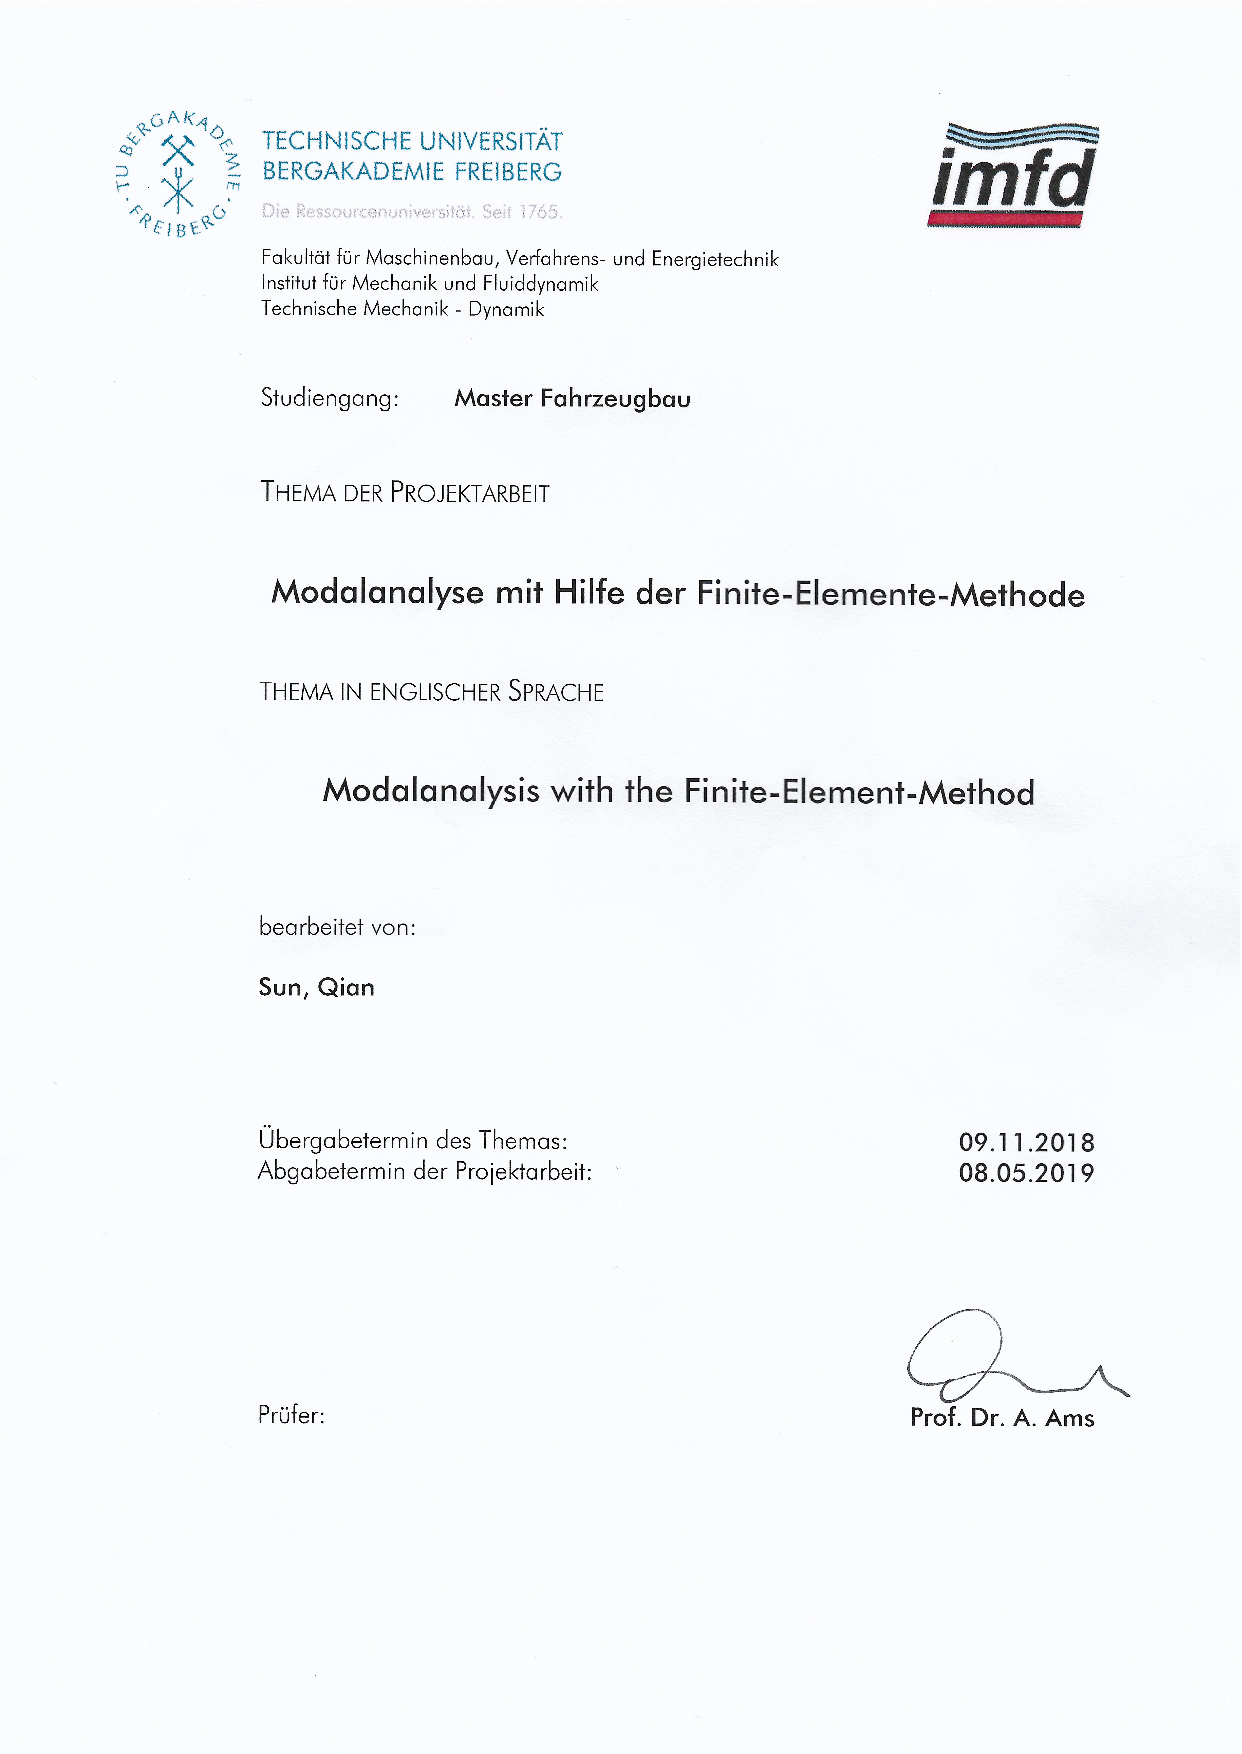
\includepdf{Deckblatt.pdf}
	
% empty page %%%%%%%%%%%%%%%%%%%
	\newpage
	\pagestyle{empty}
		\ \\
		\newpage
	\pagestyle{fancy}
%%%%%%%%%%%%%%%%%%%%%%%%%%%%%%%
	
% Erklärung %%%%%%%%%%%%%%%%%%%%%%%%%%%%%%%%%%%%%%%%%%%%%%%%%%%%%%%%%%%%%
	{\LARGE \textbf{Erklärung}}\\
	
	Hiermit versichere ich, die vorliegende Arbeit ohne Hilfe Dritter und nur mit den angegebenen
	Quellen und Hilfsmitteln angefertigt zu haben. Alle Stellen, die aus den Quellen entnommen
	wurden, sind als solche kenntlich gemacht worden. Diese Arbeit hat in gleicher oder ähnlicher
	Form noch keiner Prüfungsbehörde vorgelegen.\\
	\\
	\\
	\\
	\\
	Freiberg, den\underline{\quad \quad}.\underline{\quad \quad}.20\underline{\quad \quad}\\
	\\
	\\
	\\
	\underline{\qquad \qquad \qquad \qquad \qquad \quad} \\
	(Vorname Name)
%%%%%%%%%%%%%%%%%%%%%%%%%%%%%%%%%%%%%%%%%%%%%%%%%%%%%%%%%%%%%%%%%%%%%%%%%%%%%%%%%%%%%%%%%%%%%%%%%%%


	\newpage
	\pagestyle{empty}
	\ \\
	\newpage
	
	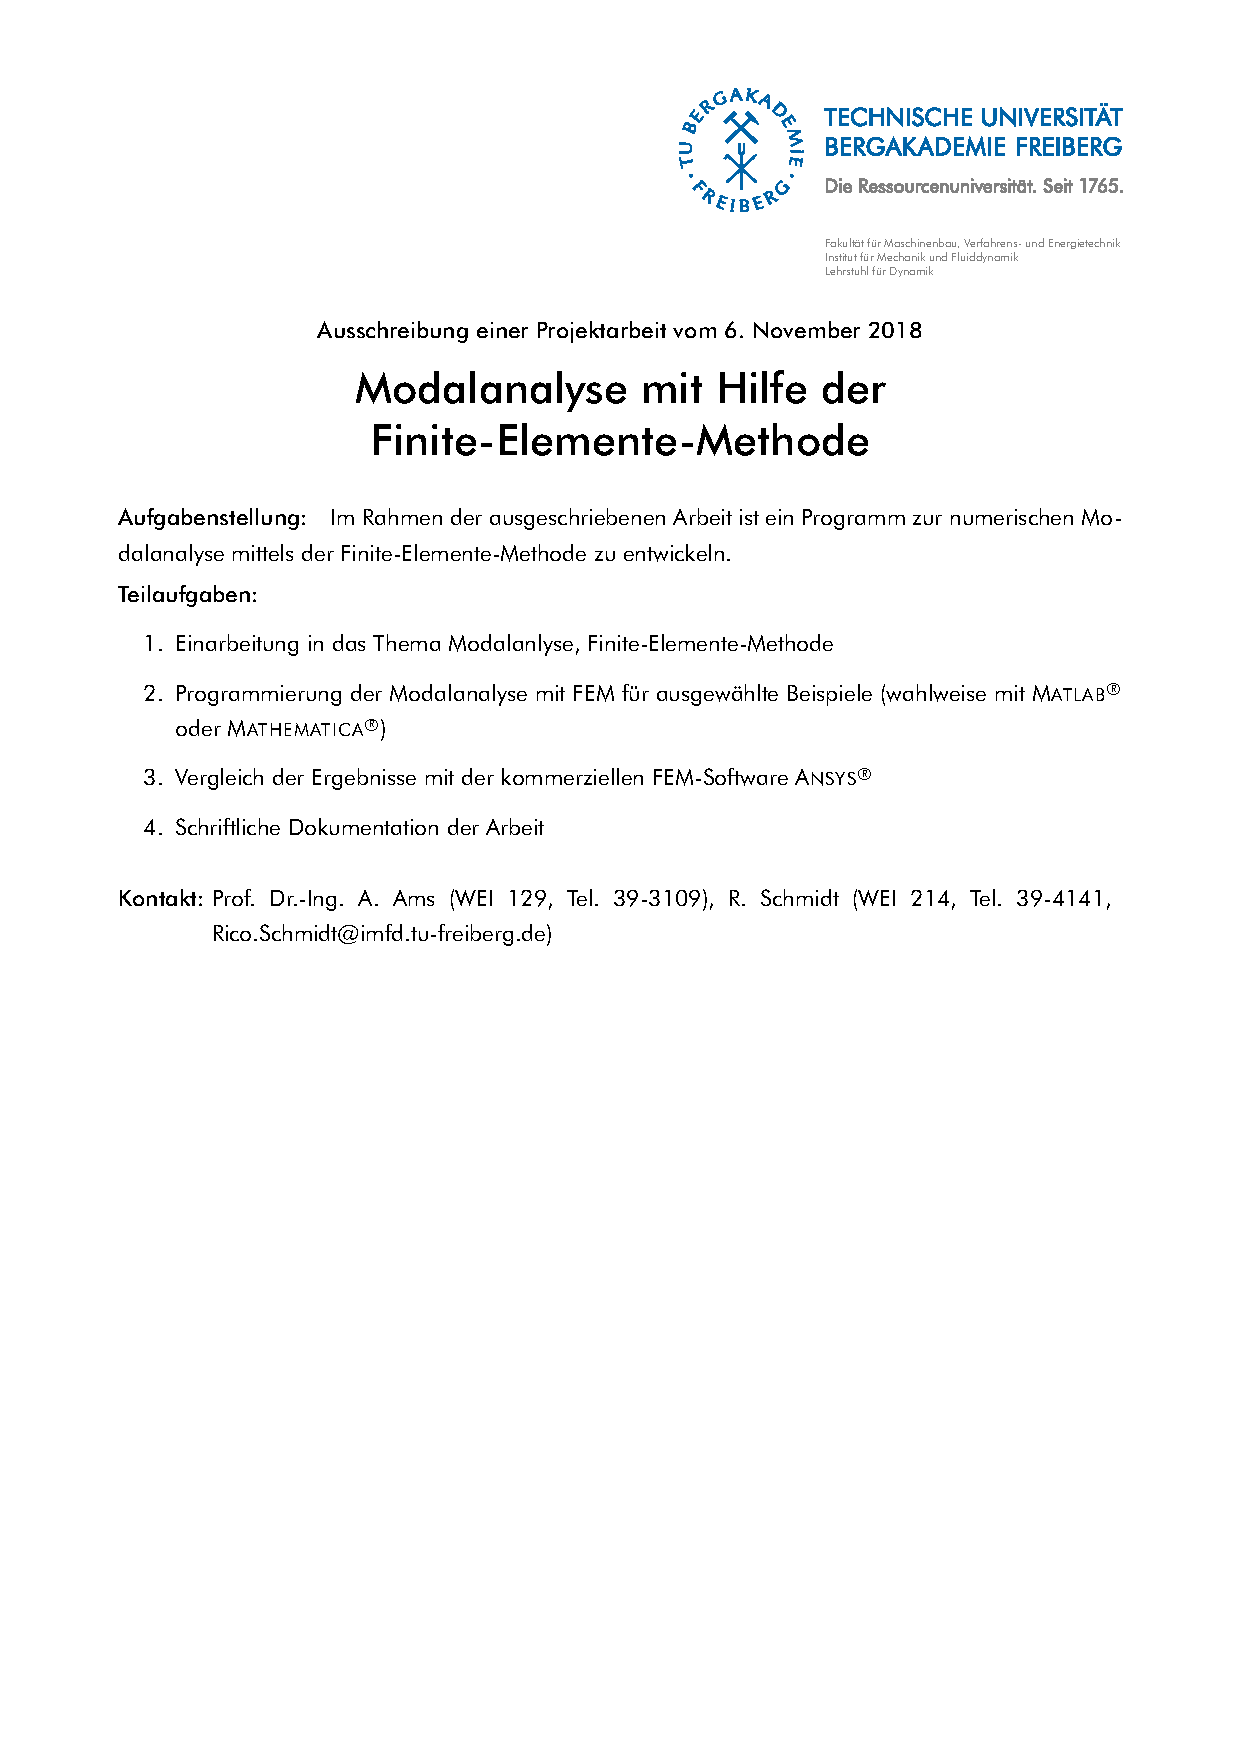
\includepdf{Ausschreibung_PA.pdf}
	
%% empty page %%%%%%%%%%%%%%%%%%%%%%%%%%%%%%%%%%%%%%%%%%
	\newpage
	\pagestyle{empty}
	\ \\
	\newpage
%%%%%%%%%%%%%%%%%%%%%%%%%%%%%%%%%%%%%%%%%%%%%%%%%%%%%%%%%

	\end{titlepage}
	
	\newpage
	
% Contents %%%%%%%%%%%%%%%%%%%%%%%%%%%%%%%%%%%%%%%%%%%%%%%%%%%%%%%%%%%%%%%%%%%%%%%%%%%%%%%%%%%%%
	
    \pagestyle{fancy}
	\fancyhead[LO,RE]{\thepage}%Kopfzelle - ungrade Seite links und grade Seite rechts - show pagenumber
	
	\tableofcontents
	
%% empty page %%%%%%%%%%%%%%%%%%%%%%%%%%%%%%%%%%%%%%%%%%
	\newpage
	\pagestyle{empty}
	\ \\
	\newpage	
%%%%%%%%%%%%%%%%%%%%%%%%%%%%%%%%%%%%%%%%%%%%%%%%%%%%%%%%%%%%%%%%%%%%%%%%%%%%%%%%%%%%%%%%%%%%%%%%%%%%%%%%%%%%%%%%%%
	
% Symbol- und Abkürzungsverzeichnis %%%%%%%%%%%%%%%%%%%%%%%%%%%%%%%%%%%%%%%%%%%%%%%%%%%%%%%%%%%%%%%%%%%%%%%%%%%%%%%%%%%%%%%%%%%%%%%
		\pagestyle{fancy}
	\fancyhead[RO,LE]{Symbol- und Abkürzungsverzeichnis}
	\section*{Symbol- und Abkürzungsverzeichnis}

	\subsection*{Lateinische Notation}
	\begin{flalign*}
	& A       && \text{m}^{2}    && \text{Querschnittfläche}    && \\
	& b       && \text{m}        && \text{Breit des Querschnitts}    && \\
	& B       && \text{m}        && \text{Breit der Platte}    && \\
	& E       && \text{N}/\text{mm}^{2} && \text{E-Modul} && \\
	& E_{kin} && \text{J}        && \text{kinetische Energie} && \\
	& E_{pot} && \text{J}        && \text{potentielle Energie} && \\
	& f       && \mathrm{Hz}      && \text{Eigenfrequenz}    && \\
	& h       && \text{m}        && \text{Höhe des Querschnitts}    && \\
	& H       && \text{m}        && \text{Dicke der Platte}    && \\
	& i,k     && -        && \text{Zählvariablen}    && \\
	& I       && \text{m}^{4}    && \text{Flächenträgheitsmoment}    && \\
	& l       && \text{m}        && \text{Länge}    && \\
	& l_{e}   && \text{m}        && \text{Länge eines Elements}    && \\
	\end{flalign*}



	
	\subsection*{Griechische Notation}
	\begin{flalign*}
	& \varepsilon && -        && \text{Dehnung}    && \\
	& \lambda     && -        && \text{Eigenwert}    && \\
	& \nu         && -        && \text{Poissionzahl}    && \\
	& \rho        && \text{kg}/\text{m}^{3} && \text{Dichte}    && \\
	\end{flalign*}

	
	\subsection*{Vektoren und Matrizen}
	\begin{flalign*}
	& \mathbf{D}      && \text{Dämpfungsmatrix}    && \\
	& \mathbf{K}      && \text{Steifigkeitsmatrix}    && \\
	& \mathbf{M}      && \text{Massenmatrix}    && \\
	& \mathbf{K}_{e}  && \text{Steifigkeitsmatrix eines Elements}    && \\
	& \mathbf{M}_{e}  && \text{Massenmatrix eines Elements}    && \\
	& \vec{N}         && \text{Vektor der Formfunktion}    && \\
	& u(x,t)          && \text{Längsverschiebung}    && \\
	& w(x,t)          && \text{Durchbiegung}    && \\
	% & \vec{u} \ , \ \vec{w}          && \text{Vektor der Elementfreiheitsgrade}    && \\ 
	\end{flalign*}
	
	\subsection*{Indices}
	\begin{flalign*}
	& ( \quad )_{,t}      && \text{Erste Ableitung nach der Zeit}    && \\
	& ( \quad )_{,tt}      && \text{Zweite Ableitung nach der Zeit}    && \\
	& ( \quad )_{,x} \ ; \ (\quad)_{,y} \ ; \ (\quad)_{,z}    && \text{Erste Ableitung in Richtung x,y,z}    && \\
	& ( \quad )_{,xx} \ ; \ (\quad)_{,yy} \ ; \ (\quad)_{,zz}    && \text{Zweite Ableitung in Richtung x,y,z}    && \\
	\end{flalign*}
	
%%%%%%%%%%%%%%%%%%%%%%%%%%%%%%%%%%%%%%%%%%%%%%%%%%%%%%%%%%%%%%%%%%%%%%%%%%%%%%%%%%%%%%%%%%%%%%%%%%%%%%%%%%%%%%%%%%%%%%%%%

%% empty page %%%%%%%%%%%%%%%%%%%%%%%%%%%%%%%%%%%%%%%%%%
%	\newpage
%	\pagestyle{empty}
%	\ \\
%	\newpage
%%%%%%%%%%%%%%%%%%%%%%%%%%%%%%%%%%%%%%%%%%%%%%%%%%%%%%%%%
	
	\pagestyle{fancy}
	\fancyhead[RO,LE]{\nouppercase\leftmark} % Kopfzelle ungrade Seite rechts und gerade Seite links - show section

	
	\pagenumbering{arabic}
	\setcounter{page}{1} 
	
	\section{Einleitung}\label{sec:einleitung}
	
	Die Modalanalyse stellt die Untersuchung der dynamischen Eigenschaften von Systemen im Frequenzbereich dar. Beispiele hierfür sind das Messen der Vibrationen einer Fahrzeugkarosserie, wenn diese an einem Rüttler angebracht ist, oder das Rauschmuster in einem Raum, wenn dieser von einem Lautsprecher angeregt wird. Im konstruktiven Ingenieurbau verwendet die Modalanalyse die Gesamtmasse und Steifigkeit einer Struktur, um die Eigenfrequenzen zu ermitteln. \\
	
	Die Eigenfrequenzen sind im konstruktiven Ingenieurbau sehr wichtig, da es unerlässlich ist, dass diese nicht mit den erwarteten Erregungsfrequenzen übereinstimmen (Resonanz). Falls es trotzdem zur Resonanz kommt, kann das Objekts strukturellen Schaden erleiden. Beispielsweise wird bei Bauwerken wie Brücken versucht, die Eigenfrequenzen von den Frequenzen der auf der Brücke gehenden Personen fernzuhalten. Andere natürliche Anregungen können auch vorhanden sein und die Eigenmoden einer Brücke erregen (z.B.: Anregung durch Wind).\\
	
	Aus methodologischer Sicht ist die Modalanalyse in numerische und experimentelle Modalanalyse zu unterteilen. Wenn die Modalparameter beispielsweise durch die Finite-Elemente-Methode erhalten werden, wird sie als numerische Modalanalyse bezeichnet. Bei der experimentellen Modalanalyse werden Anregung und Antwort über Sensoren gemessen. Anschließend werden die modalen Parameter durch Parameteridentifikation analysiert.\\
	
	In dieser Arbeit wird die numerische Modalanalyse mit der Finite-Elemente-Methode betrachtet. Die Finite-Elemente-Methode ist ein allgemeines, bei unterschiedlichen physikalischen Aufgabenstellungen angewendetes numerisches Verfahren. Typische Anwendungsbereiche sind Strukturanalyse, Wärmeübertragung, Fluiddynamik, Massentransport und elektromagnetisches Potential. Der Berechnungsbereich ist in viele Teile mit einfacher Form unterteilt z.B. Quadrate oder Tetraeder. Sie sind die \glqq finiten Elemente\grqq. Ihr physikalisches Verhalten lässt sich aufgrund ihrer einfachen Geometrie mit bekannten Ansatzfunktionen gut berechnen. Das physikalische Verhalten des gesamten Körpers wird dadurch wiedergegeben, wie diese Elemente auf die Kräfte, Belastungen und Randbedingungen reagieren und wie sich Belastungen und Reaktionen beim Übergang von einem Element zum Nachbarn durch bestimmte problembezogene Steifigkeitsbedingungen ausbreiten, die die Ansatzfunktion erfüllen müssen.\\
	
	Darüber hinaus enthalten die Ansatzfunktionen die Parameter, die normalerweise eine physikalische Bedeutung haben, z. B. das Verschieben eines bestimmten Punkts in der Komponente zu einem bestimmten Zeitpunkt. Die Suche nach der Bewegungsfunktion wird somit auf die Suche nach den Werten der Parameter der Funktionen zurückgeführt. Durch die Verwendung von immer mehr Parametern (z. B. mehr und mehr kleinere Elemente) oder Ansatzfunktionen mit immer höherem Wert kann die Genauigkeit der der Näherungslösung verbessert werden.\\
	
	Um die Bewegungsgleichungen eines Körpers zu gewinnen, wird das Prinzip von \textsc{Hamilton} benutzt, das auch als das Prinzip der stationären Wirkung bezeichnet wird. Anschließend wird die FE Simulation mit \Matlab beschrieben. Außerdem werden die FE-Software \Ansys sowie analytische Lösungen nach \cite{stephan1995schwingungen} zum Vergleichen der Ergebnisse benutzt.
	
%% empty page %%%%%%%%%%%%%%%%%%%%%%%%%%%%%%%%%%%%%%%%%%
	\newpage
	\pagestyle{empty}
	\ \\
	\newpage
%%%%%%%%%%%%%%%%%%%%%%%%%%%%%%%%%%%%%%%%%%%%%%%%%%%%%%%%%
	\pagestyle{fancy}
	\section{Theoretische Grundlagen} \label{sec:Theoretische Grundlagen}
	\subsection{Grundlagen der Finite-Elemente-Methode}\label{sec:Grundlagen-FEM}
	Die Finite-Elemente-Methode (FEM) ist eine numerische Methode zur Lösung von Problemen der Ingenieurwissenschaften und der mathematischen Physik. FEM ist eine leistungsstarke, häufig verwendete Berechnungsmethode, die zu einem System algebraische Gleichungen führt. Die Methode nähert sich der unbekannten Funktion über das Grundgebiet an. Um das Problem zu lösen, wird ein großes System in kleinere, einfachere Teile unterteilt, die als finite Elemente bezeichnet werden. Die einfachen Gleichungen, die diese finiten Elemente modellieren, werden dann zu einem größeren Gleichungssystem zusammengefügt, das das gesamte Problem beschreibt. Die FEM verwendet Methoden aus der Variationsrechnung, um eine Lösung anzunähern, indem der zugehörige Fehler minimiert wird.\\
	
	Die Unterteilung des ganzen Gebiets in einfachere Teile hat mehrere Vorteile:
	\begin{itemize}
		\item Darstellung von komplexen Geometrien,
		\item Einbeziehung unterschiedlicher Materialeigenschaften,
		\item Einfache Darstellung der Gesamtlösung,
		\item Erfassung von lokalen Auswirkungen.
	\end{itemize}
	
	Ein typischer Vorgang des Verfahrens umfasst:
	\begin{enumerate}
		\item Das Unterteilen (\textit{Diskretisieren}) des ganzen Grundgebiets des Problems in eine Sammlung von einfachen Teilgebieten, die sogenannten finiten Elemente, wobei jedes Teilgebiet durch eine Reihe von Elementgleichungen für das ursprüngliche Problem repräsentiert wird.
		\item Systematische Rekombination aller Elementgleichungen zu einem globalen Gleichungssystem für die endgültige Berechnung. Das globale Gleichungssystem hat eine bekannte Lösungsmethode und kann aus den Anfangswerten des ursprünglichen Problems berechnet werden, um eine numerische Lösung zu erhalten.
	\end{enumerate}
	
	Im ersten Schritt handelt es sich bei den Elementgleichungen um einfache Gleichungen, die sich lokal den zu untersuchenden ursprünglichen komplexen Gleichungen annähern, wobei die ursprünglichen Gleichungen oft partielle Differentialgleichungen sind.\\
	
	Die Finite-Elemente-Methode diskretisiert das Grundgebiet in einen Gesamtbau endlicher Finite-Elemente. Die Ecken der Finite-Elemente werden Knoten genannt. Diese Knoten bilden die diskrete Untergruppe für die numerische Methode. Auf den Elementen werden Annäherungsfunktionen eingeführt, die die begrenzte anstehenden und unbekannten Knotengrößen als Parameter enthalten. Die resultierenden Elementintegrale werden mit numerischer Quadratur berechnet. Die Elementgleichung werden durch Kontinuitätsanforderungen an den Elementgrenzen zusammengesetzt. Auf diese Weise werden Randwertprobleme für lineare partielle Differentialgleichungen in ein lineares Gleichungssystem mit symmetrischen Systemmatrizen übertragen. Für nichtlineare Differentialgleichungen ist der Algorithmus analog mit dem Unterschied, dass nichtlineare Abhängigkeiten unter Verwendung geeigneter Verfahren (z.B. \textsc{Newton}-Verfahren) iterativ linearisiert werden und das lineare Gleichungssystem in jedem inkrementellen Schritt eingerichtet wird.\\
	
	Für bestimmte Aufgaben ist die Unterteilung in Elemente durch das Problem bereits weitgehend vorbestimmt, beispielsweise bei räumlichen Fachwerken, bei denen die einzelnen Stäbe die Konstruktionselemente bilden. Bei zweidimensionalen Problemen wird das Grundgebiet z. B. in Dreiecke oder Vierecke unterteilt. Räumliche Probleme werden behandelt, indem das dreidimensionale Gebiet in Tetraederelemente, Quader oder andere an das Problem angepasste Elemente, möglicherweise auch gekrümmt, unterteilt wird. \\
	
	Im zweiten Schritt wird ein globales Gleichungssystem aus den Elementgleichungen durch eine Transformation der Koordinaten von den lokalen Knoten der Teilgebiete zu den globalen Knoten des Gesamtgebiets generiert. Diese räumliche Transformation enthält geeignete Abbildungsmatrizen, die in Bezug auf das Koordinatensystem angewendet werden.\\
	
	In jedem der Elemente wird für die gesuchte Funktion, bzw. allgemeiner für die das Problem beschreibenden Funktionen, ein problemgerechter Ansatz gewählt. Im Besonderen eignen sich dazu ganze rationale Funktionen in den unabhängigen Raumkoordinaten.
	Für eindimensionale Elemente (Stäbe, Balken) kommen Polynome ersten, zweiten, dritten und gelegentlich sogar höheren Grades in Frage. Bei zweidimensionalen Problemen finden lineare, quadratische oder höhergradige Polynome Verwendung \cite{schwarz2013methode}. \\
	
	Strukturmechanische FEM-Systeme werden durch lineare Gleichungssysteme 2. Ordnung
	\begin{equation}\label{equ:FEM-Ansatzgleichung}
	\mathbf{M}\, \ddot{u}(t)+ \mathbf{D}\, \dot{u}(t)+ \mathbf{K}\, u(t) = P(t)
	\end{equation}
	dargestellt.
	$ \mathbf{M} $ , $ \mathbf{D} $ und $ \mathbf{K} $ sind die Massen-, Dämpfungs- und Steifigkeitsmatrix des Systems und $ P(t) $ ist der Vektor der externen Kräfte, die auf das System wirken.  Der Vektor der Freiheitsgrade ist mit $ u(t) $ gegeben. Um die verschiedenen Matrizen zu berechnen, werden unterschiedliche physikalische oder energetische Prinzipien verwendet, wie z. B. in dieser Arbeit das Prinzip von \textsc{Hamilton}.
	
	\subsection{Prinzip von Hamilton} \label{sec:prinzip-hamilton}
	In der Physik ist das Prinzip von \textsc{Hamilton} der Ausdruck des 1833 vom irischen Physiker \textsc{William Hamilton} veröffentlichten Prinzips. Das Prinzip von \textsc{Hamilton} besagt, dass die Dynamik eines physikalischen Systems mittels Variationsrechnung einer einzigen Funktion, der \textsc{Lagrange}-Funktion welche alle physikalischen Informationen über das System und die darauf einwirkenden Kräfte enthält, bestimmt wird. \\
	
	Die \textsc{Lagrange}-Funktion, auch \textsc{Lagrange}-Größe genannt, enthält alle physikalischen Konnotationen dieses physischen Systems. Für ein Partikelsystem mit einem generalisierten Potential und Zwangsbedingungen lautet die \textsc{Lagrange}-Funktion
	\begin{equation}\label{equ:lagrange-funktion}
	L = E_{kin} - E_{pot} \, ,
	\end{equation}
	wobei $ E_{kin} $  die gesamte kinetische Energie und $ E_{pot} $ die potentielle Energie des Systems sind. \\
	
	Die kinetische Energie eines Objekts ist die Energie, die es aufgrund seiner Bewegung besitzt. Diese Energie wird als die Arbeit definiert, die erforderlich ist, um einen Körper einer bestimmten Masse von der Ruhe auf seine vorgegebene Geschwindigkeit zu beschleunigen. Nachdem der Körper diese Energie während seiner Beschleunigung gewonnen hat, erhält er diese kinetische Energie aufrecht, wenn sich seine Geschwindigkeit nicht ändert. Die gleiche Arbeit wird vom Körper geleistet, wenn er von seiner aktuellen Geschwindigkeit in einen Ruhezustand verlangsamt wird.\\
	
	In der klassischer Mechanik hängt die kinetische Energie eines Punktobjekts oder eines nicht-rotierenden starren Körpers von der Masse des Körpers und seiner Geschwindigkeit ab. \\
%	Die kinetische Energie ist
%	\begin{equation}\label{equ:kin-energi}
%	E_{kin} = \frac{1}{2} m v^{2} \, .
%	\end{equation}	

	Übliche Arten von potentieller Energie umfassen die potentielle Schwerkraftenergie eines Objekts, die von seiner Masse und seinem Abstand vom Massenschwerpunkt eines anderen Objekts abhängt, der elastischen potentiellen Energie einer ausgedehnten Feder und der elektrischen potentiellen Energie.\\	
	
	Das Prinzip von \textsc{Hamilton} ist auch ein wichtiges Variationsprinzip in der Elastodynamik. Im Gegensatz zu einem System, das aus starren Körper besteht, haben verformbare Körper unendlich viele Freiheitsgrade und besetzen ununterbrochene Raumregionen. Der Zustand des Systems wird daher durch kontinuierliche Funktionen von Raum und Zeit beschrieben. Das erweiterte Prinzip von \textsc{Hamilton} für solche Körper wird durch
	\begin{equation}\label{equ:Hamilton}
	\delta\int_{t_{1}}^{t_{2}} \left( E_{kin}-E_{pot}\right)  \mathrm{d}t + \int_{t_{1}}^{t_{2}} \delta W \mathrm{d}t = 0
	\end{equation}
	gegeben.
	Nacheinander sind also die kinetische Energie $ E_{kin} $ und die potenzielle Energie $ E_{pot} $ des Systems sowie die virtuelle Arbeit $ \delta W $ aller angreifenden potentiallosen Kräfte, zugeschnitten auf das zu betrachtende ein- oder zweiparametrige Strukturmodell, zu bestimmen. \cite{wauer2014kontinuumsschwingungen}
	
	\clearpage
	
%% empty page %%%%%%%%%%%%%%%%%%%%%%%%%%%%%%%%%%%%%%%%%%
	\newpage
	\pagestyle{empty}
	\ \\
	\newpage
%%%%%%%%%%%%%%%%%%%%%%%%%%%%%%%%%%%%%%%%%%%%%%%%%%%%%%%%%
	\pagestyle{fancy}
	\section{Finite-Elmenete und Matrizen} \label{sec:eindimensional-fall}
	
	Jedes Element vom Grundgebiet hat ein eigenes lokales Koordinatensystem. Die lokalen Koordinaten eines Elements sind von -1 bis +1 definiert. Die globale Länge eines Elements ist $ l_{e} $.\\
	Zunächst soll die Transformation von der lokalen Variable $\xi$ mit dem Intervall $[-1,1]$ auf die globale Koordinate $x$ mit dem Intervall $ [0,l_{e}] $ mit 
	\begin{equation}\label{equ:lokal-zu-global}
	\left. 
	\begin{array}{l}
	\xi (x) = a_{0} + a_{1}x\\
	\xi (x=0) \overset{!}{=} -1\\
	\xi (x=l_{e})  \overset{!}{=} 1
	\end{array} 
	\right\rbrace \Rightarrow 
	\xi = -1 + \frac{2}{l_{e}}x
	\Rightarrow
	\frac{\partial \xi}{\partial x} = \frac{2}{l_{e}}
	\end{equation}
	beschrieben werden.
	
	\subsection{Stabelemente}\label{sec:längsschwingung-von-stab}
	Für ein ungedämpftes Stabelement lautet die potentielle Energie in Abhängigkeit der Längsverschiebung
	 $ u(x,t) $
	\begin{equation}\label{equ:Stab-pot-Energie}
	E_{pot} = \frac{1}{2} \int_{0}^{l_{e}} EA u_{,x}^{2} \mathrm{d}x,
	\end{equation}
	
	die kinetische Energie
	\begin{equation}\label{equ:Stab-kin-Energie}
	E_{kin} = \frac{1}{2} \int_{0}^{l_{e}} \rho A u_{,t}^{2} \mathrm{d}x
	\end{equation}
	
	und die virtuelle Arbeit der potentiallosen Kräfte
	\begin{equation}\label{equ:Stab-virt-Arbeit}
	\delta W = 0.
	\end{equation}
	
	Mit dem Prinzip von \textsc{Hamilton} (Gleichung \ref{equ:Hamilton}) ergibt sich
	\begin{equation}\label{equ:Stab-Hamilton}
	\delta \int_{t_{0}}^{t_{1}} \int_{0}^{l_{e}} \frac{1}{2} \rho A u_{,t}^{2} - \frac{1}{2} E A u_{,x}^{2} \mathrm{d}x \mathrm{d}t = 0
	\end{equation}
	
	und nach der Variation sowie partiellen Integration

	\begin{equation}\label{equ:Stab-Hamilton-Formulierung}
	\int_{t_{0}}^{t_{1}} \int_{0}^{l_{e}} \rho A u_{,tt} \delta u + E A u_{,x} \delta u_{,x} \mathrm{d}x \mathrm{d}t = 0.
	\end{equation}
	
	Dabei handelt es sich um die schwache Formulierung der Bewegungsdifferentialgleichung des Dehnstabes. Für die Ortsdiskretisierung dieser Gleichung werden folgende Ansätze
	\begin{equation}\label{equ:Stab-Hamilton-variiert}
	\begin{aligned}
	&u(x,t) &=& \vec{N}(x) \vec{u}(t); &  \delta u(x,t) &=& \vec{N}(x) \delta \vec{u}(t) \\
	&u_{,x}(x,t) &=& \vec{N}_{,x}(x) \vec{u}_{,tt}(t);  & \delta u_{,x}(x,t) &=& \vec{N}_{,x}(x) \delta \vec{u}(t)  \\
	&u_{,t}(x,t) &=& \vec{N}(x) \vec{u}_{,t}(t)\\
	&u_{,tt}(x,t) &=& \vec{N}(x) \vec{u}_{,tt}(t)  
	\end{aligned}
	\end{equation}
	verwendet. Die Vektoren für die Formfunktionen und die Elmenetfreiheitsgrade sind mit $\vec{N}(x)$ und $\vec{u}(t)$ gegeben. Zusammen mit Gleichung (\ref{equ:Stab-Hamilton-Formulierung}) ergibt sich
	\begin{equation}\label{equ:Stab-Hamilton-end}
	\int_{t_{0}}^{t_{1}} \int_{0}^{l_{e}} \left[ \rho A \vec{N}^{T}(x) \vec{N}(x) \vec{u}_{,tt}(t) + E A \vec{N}_{,x}^{T}(x) \vec{N}_{,x}(x) \vec{u}(t) \right] \mathrm{d}x \delta \vec{u}(t) \mathrm{d}t = 0.
	\end{equation}
	Die Massenmatrix eine Elements lässt sich mit
	\begin{equation}\label{equ:Stab-Me-Matrix}
	\mathbf{M}_{e} = \int_{0}^{l_{e}} \rho A \vec{N}^{T}(x) \vec{N}(x) \mathrm{d}x
	\end{equation}
	
	und die Steifigkeitsmatrix mit
	\begin{equation}\label{equ:Stab-Ke-Matrix}
	\mathbf{K}_{e} = \int_{0}^{l_{e}} E A \vec{N}_{,x}^{T}(x) \vec{N}_{,x}(x) \mathrm{d}x
	\end{equation}
	angeben. Nach dem Zusammenbau der Gesamtmassenmatrix $ \mathbf{M} $ und Gesamtsteifigkeitsmatrix $ \mathbf{K} $ aus den  Elementmatrizen ergibt sich das FE-Gleichungssystem für den ungedämpften Stab zu
	\begin{equation}\label{equ:Ausgangspunkt}
	\mathbf{M} \cdot \ddot{\vec{q}}(t) + \mathbf{K} \cdot \vec{q}(t) = 0
	\end{equation}
	Der Vektor $\vec{q}(t)$ beinhaltet dabei sämtliche Knotenfreiheitsgrade. Durch die Definition der Zusatndsgrößen
	\begin{equation}\label{equ:Ansatz-in-Systemmatrix}
	\left. 
	\begin{array}{c}
	\vec{z}_{1} = \vec{q} \\
	\vec{z}_{2} = \dot{\vec{q}}
	\end{array}
	\right\rbrace \Rightarrow	
	\begin{array}{l}
	\dot{\vec{z}}_{1} = \vec{z}_{2} \\
	\dot{\vec{z}}_{2} = \ddot{\vec{q}} = - \mathbf{M}^{-1} \cdot \mathbf{K} \cdot \vec{x} = - \mathbf{M}^{-1} \cdot \mathbf{K} \cdot \vec{z}_{1}
	\end{array}
	\end{equation}
	kann Gleichung \eqref{equ:Ausgangspunkt} im Zusatndsraum 
	\begin{equation}\label{equ:1st-Ausgangspunkt}
	\left[ 
	\begin{array}{c}
	\dot{\vec{z}}_{1}\\
	\dot{\vec{z}}_{2}
	\end{array}
	\right] 
	=
	\left[ 
	\begin{array}{cc}
	\mathbf{0}                        & \mathbf{E} \\
	-\mathbf{M}^{-1} \cdot \mathbf{K} & \mathbf{0}
	\end{array}
	\right]
	\cdot
	\left[ 
	\begin{array}{c}
	\vec{z}_{1}\\
	\vec{z}_{2}
	\end{array}
	\right] 
	\end{equation}
	angegeben werden. Die Eigenfrequenzen des Stabes können durch die Eigenwerte der Systemmatrix
	\begin{equation}\label{equ:Systemmatrix}
	\mathbf{A}
	=
	\left[ 
	\begin{array}{cc}
	\mathbf{0}                        & \mathbf{E} \\
	-\mathbf{M}^{-1} \cdot \mathbf{K} & \mathbf{0}
	\end{array}
	\right]
	\end{equation}
	bestimmt werden.
	
	\subsubsection{Linearer Ansatz} \label{sec:linealischer ansatz}
	Für die Längsverschiebung $ u(\xi) $ eines Elements soll ein linearer Ansatz der Form
	\begin{equation}\label{equ:linear-Einsatz}
	u(\xi)=a_{0}+a_{1}\xi
	\end{equation}
	verwendet werden. Zur Bestimmung der Koeffizienten $a_{i}$ wird
	\begin{equation}\label{equ:linear-Einsatz-Forderung}
	u(-1) \overset{!}{=} u_{1} \ ; \  u(1) \overset{!}{=} u_{2}
	\end{equation}	
	gefordert. Die Knotenverschiebungen $u_{i}(t)$ sind dabei Zeitfunktionen. Damit ergibt sich Gleichung \eqref{equ:linear-Einsatz} zu
	\begin{equation}\label{equ:linear-Einsatz-eingesetzt}
	u(\xi,t)=\frac{u_{1}+u_{2}}{2} + \frac{1}{2} (-u_{1}+u_{2})\xi
	\end{equation}
	bzw. in Vektor-Matrix Schreibweise
	\begin{equation}\label{equ:linear-Einsatz-Algebra}
	u(\xi,t) = \vec{N}(\xi) \vec{u}(t) =
	\left[ \begin{array}{cc}
	\frac{1}{2} - \frac{\xi}{2} & \frac{1}{2} + \frac{\xi}{2}
	\end{array} \right]	
	\left[ 
	\begin{array}{c}
	u_{1}\\
	u_{2}
	\end{array} 
	\right] .
	\end{equation}
	Die Ableitung der Funktion $ u(\xi,t) $ nach der globalen Variable $x$ erfolgt mit
	\begin{equation}\label{equ:stab-ux-Ableitung}
	u_{,x}(\xi,t)= \frac{\partial}{\partial x} [\vec{N}(\xi) \vec{u}(t) ] = \frac{\partial}{\partial x} \frac{\partial \xi}{\partial \xi} [\vec{N}(\xi) \vec{u}(t)] =  \frac{\partial \vec{N}(\xi)}{\partial \xi} \cdot \frac{\partial \xi}{\partial x} \cdot \vec{u}(t).
	\end{equation}
	Mit dem Zusammenhang zwischen globaler und lokaler Koordinate \eqref{equ:lokal-zu-global} ergibt sich
	\begin{equation}\label{equ:linear-N-x-Ableitung}
	\vec{N}_{,x}(\xi) = \frac{\partial \vec{N}(\xi)}{\partial \xi} \cdot \frac{\partial \xi}{\partial x} =
	\left[
	\begin{array}{c c} 
	-\frac{1}{2} & +\frac{1}{2} 
	\end{array}
	\right]
	\cdot \frac{2}{l_{e}}.
	\end{equation}
	Die Elementmassenmatrix des $i$-ten Elements (Größe 2x2) ist mit
	\begin{equation}\label{equ:linear-Mei-matrix}
	\mathbf{M}_{ei} = \left[ 
	\begin{array}{cc}
	M_{ei,11} & M_{ei,12} \\
	M_{ei,21} & M_{ei,22}
	\end{array}
	\right] 
	\end{equation}
	gegeben. Damit kann die Gesamtmassenmatrix nach
	\begin{equation}\label{equ:linear-M-Matrix}
	\mathbf{M} = 
	\left[ 
	\begin{array}{ccccc}
	M_{e1,11} & M_{e1,12}           & 0                   & 0                   & \cdots \\
	M_{e1,21} & M_{e1,22}+M_{e2,11} & M_{e2,12}           & 0                   & \cdots \\
	0         & M_{e2,21}           & M_{e2,22}+M_{e3,11} & M_{e3,12}           & \cdots \\
	0         & 0                   & M_{e3,21}           & M_{e3,22}+M_{e4,11} & \cdots \\
	\colon    & \colon              & \colon              & \colon              & \ddots 
	\end{array}
	\right] 
	\end{equation}
	zusammengebaut werden. Nach gleicher Regel wird auch die Gesamtsteifigkeitsmatrix $ \mathbf{K} $ berechnet.
	
	\subsubsection{Quadratischer Ansatz} \label{sec:quadratischer ansatz}
	Ausgangspunkt ist der quadratische Ansatz
	\begin{equation}\label{equ:quadra-ansatz}
	u(\xi) = a_{0} + a_{1} \xi + a_{2} \xi^{2}
	\end{equation}
	mit den Forderungen
	\begin{equation}\label{equ:quadra-ansatz-forderungen}
	u(-1) \overset{!}{=} u_{1} \ ; \ u(0) \overset{!}{=} u_{2} \ ; \ u(+1) \overset{!}{=} u_{3}.
	\end{equation}
	Nach Auswertung der Forderungen ergibt sich Gleichung (\ref{equ:quadra-ansatz}) in Abhängikeit der Knotenverschiebungen $u_{i}(t)$ zu
	\begin{equation}\label{equ:quadra-ansatz-eingestzt}
	u(\xi,t) = \vec{N}(\xi) \vec{u}(t) =
	\left[ 
	\begin{array}{ccc}
	\frac{\xi^{2}}{2}-\frac{\xi}{2} & 1-\xi^{2} & \frac{\xi}{2}+\frac{\xi^{2}}{2}
	\end{array}
	\right] 
	\left[ 
	\begin{array}{c}
	u_{1} \\
	u_{2} \\
	u_{3}
	\end{array}
	\right] .
	\end{equation}
	Die Ableitung des Vektors der Formfunktionen lautet
	\begin{equation}\label{equ:qudra-N-ableitung}
	\vec{N}_{,x}(x) =\frac{\partial \vec{N}(\xi)}{\partial x}= \frac{\partial \vec{N}(\xi)}{\partial \xi} \cdot \frac{\partial \xi}{\partial x} =
	\left[ 
	\begin{array}{ccc}
	\xi - \frac{1}{2} & -2\xi & \frac{1}{2} + \xi
	\end{array}
	\right] \cdot \frac{2}{l_{e}}.
	\end{equation} 
	
	Die Elementmassenmatrix des $i$-ten Elements (Größe 3x3) ist mit
	\begin{equation}\label{equ:qudra-Kei-matrix}
	\mathbf{M}_{ei} =
	\left[ 
	\begin{array}{ccc}
	M_{ei,11} & M_{ei,12} & M_{ei,13} \\
	M_{ei,21} & M_{ei,22} & M_{ei,23} \\
	M_{ei,31} & M_{ei,33} & M_{ei,33} 
	\end{array} 
	\right] 
	\end{equation}
	gegeben. Damit kann die Gesamtmassenmatrix nach
	\begin{equation}\label{equ:qudra-K-matrxi}
	\mathbf{M} = 
	\left[ 
	\begin{array}{cccc}
	M_{e1,11} & M_{e1,12} & M_{e1,13}           & \cdots \\
	M_{e1,21} & M_{e1,22} & M_{e1,23}           & \cdots \\
	M_{e1,31} & M_{e1,32} & M_{e1,33}+M_{e2,11} & \cdots \\
	\colon    & \colon    & \colon              & \ddots 
	\end{array}
	\right] 
	\end{equation}
	zusammengebaut werden. Nach gleicher Regel wird auch die Gesamtsteifigkeitsmatrix $ \mathbf{K} $ berechnet.
	
	\subsection{Balkenelemente} \label{sec:biegeschwingung-von-balken}
	
	Für ein ungedämpftes Balkenelement lautet die kinetische Energie in Abhängigkeit der Durchbiegung $w(x,t)$
	\begin{equation}\label{equ:balken-kin-energie}
	E_{kin} = \frac{\rho A}{2} \int_{0}^{l_{e}} w_{,t}^{2} \ \mathrm{d}x,
	\end{equation}
	die potenzielle Energie
	\begin{equation}\label{equ:balken-pot-energie}
	E_{pot} = \frac{1}{2} \int_{0}^{l_{e}} E I w_{,xx}^{2} \ \mathrm{d}x
	\end{equation}
	und die virtuelle Arbeit der potentiallosen Kräfte
	\begin{equation}\label{equ:balken-virt-arbeit}
	\delta W = 0.
	\end{equation}
	Mit dem Prinzip von \textsc{Hamilton} (Gleichung \ref{equ:Hamilton}) ergibt sich
	\begin{equation}\label{equ:balken-hamilton}
	\delta \frac{1}{2} \int_{t_{0}}^{t_{1}} \int_{0}^{l_{e}} \rho A w_{,t}^{2} - EI w_{,xx}^{2} \ \mathrm{d}x \mathrm{d}t = 0
	\end{equation}
	und nach der Variation sowie partiellen Integration
	\begin{equation}\label{equ:balken-hamilton-form}
	\int_{t_{0}}^{t_{1}} \int_{o}^{l_{e}} \rho A w_{,tt} \delta w + EI  w_{,xx} \delta w_{,xx} \ \mathrm{d}x \mathrm{d}t =0.
	\end{equation}
	Die schwache Formulierung der Bewegungsdifferentialgleichung eines Biegebalkens wird mit den Ansätzen
	\begin{equation}\label{equ:balken-hamilton-ansatz}
	\begin{aligned}
	&w(x,t) &=& \vec{N}(x) \vec{w}(t);	&\delta w(x,t) &=& &\vec{N}(x) \delta\vec{w}(t)\\
	&w_{,x}(x,t) &=& \vec{N}_{,x}(x) \vec{w}(t); &\delta w_{,x}(x,t) &=& &\vec{N}_{,x}(x) \delta\vec{w}(t)\\
	&w_{,xx}(x,t) &=& \vec{N}_{,xx}(x) \vec{w}(t); &\delta w_{,xx}(x,t) &=& &\vec{N}_{,xx}(x) \delta\vec{w}(t)\\
	&w_{,t}(x,t) &=& \vec{N}(x) \vec{w}_{,t}(t)\\
	&w_{,tt}(x,t) &=& \vec{N}(x) \vec{w}_{,tt}(t)
	\end{aligned}
	\end{equation}
	ortsdiskretisiert. Zusammen mi Gleichung (\ref{equ:balken-hamilton-form}) ergibt sich
	\begin{equation}\label{equ:balken-hamilton-end}
	\int_{t_{0}}^{t_{1}} \int_{0}^{l_{e}} \left[ \rho A \vec{N}^{T}(x) \vec{N}(x) \vec{w}_{,tt}(t) + EI \vec{N}_{,xx}^{T}(x) \vec{N}_{,xx}(x) \vec{w}(t) \right] \mathrm{d}x \,\delta\vec{w}(t) \, \mathrm{d}t = 0.
	\end{equation}
	Die Massenmatrix $ \mathbf{M}_{e} $ eines Elements ist mit
	\begin{equation}\label{equ:balken-Me-matrix}
	\mathbf{M}_{e} = \int_{0}^{l_{e}} \rho A \vec{N}^{T}(x) \vec{N}(x) \mathrm{d}x
	\end{equation}
	und die Steifigkeitsmatrix $ \mathbf{K}_{e} $ mit
	\begin{equation}\label{equ:balken-Ke-matrix}
	\mathbf{K}_{e} = \int_{0}^{l_{e}} EI \vec{N}_{,xx}^{T}(x) \vec{N}_{,xx}(x) \mathrm{d}x
	\end{equation}
	gegeben. Der Übergang zum Zustandsraum und die Angbabe der Systemmatrix ist analog wie für den Dehnstab in Abschnitt \textbf{\ref{sec:längsschwingung-von-stab}} beschrieben (Gleichungen \ref{equ:Ausgangspunkt} und \ref{equ:Systemmatrix}). Die Eigenwerte und Eigenvektoren der Systemmatrix liefern wieder die Eigenfrequenzen und Eigenschwingformen des Balkens.

	
	\subsubsection{Kubischer Ansatz} \label{sec:kubischer ansatz}
	Mit einem kubischen Ansatz für die Funktion $ w(\xi) $ lässt sich ein auch für die Balkenbiegung konformes Element gewinnen, wenn neben den Funktionswerten auch noch die ersten Ableitung in den Endpunkten als Knotenvariable eingeführt werden. Es wird die Ansatzfunktion
	\begin{equation}\label{equ:kubik-ansatz}
	w(\xi) = a_{0} + a_{1}\xi + a_{2}\xi^{2} + a_{3}\xi^{3}
	\end{equation}
	verwendet und  zur Bestimmung der Koeffizienten $a_{i}$ wird
	\begin{equation}\label{equ:kubik-ansatz-forderungen}
	w(-1)\overset{!}{=}w_{1} \ ; \ w_{,\xi}(-1)\overset{!}{=}\phi_{1} \ ; \ w(+1)\overset{!}{=}w_{2} \ ; \ w_{,\xi}(+1)\overset{!}{=}\phi_{2}
	\end{equation}
	gefordert. Damit ergibt sich Gelichung (\ref{equ:kubik-ansatz}) zu 
	\begin{equation}\label{equ:kubik-ansatz-eingesetzt}
	\renewcommand\arraystretch{1.5}
	w(\xi,t) = 
	\vec{N}(\xi) \vec{w}(t)
	=
	\left[ 
	\begin{array}{c}
	-\frac{1}{16}+\frac{\xi}{16}+\frac{9\xi^{2}}{16}-\frac{9\xi^{3}}{16}\\
	\frac{9}{16}-\frac{27\xi}{16}-\frac{9\xi^{2}}{16}+\frac{27\xi^{3}}{16}\\
	\frac{9}{16}+\frac{27\xi}{16}-\frac{9\xi^{2}}{16}-\frac{27\xi^{3}}{16}\\
	-\frac{1}{16}-\frac{\xi}{16}+\frac{9\xi^{2}}{16}+\frac{9\xi^{3}}{16}
	\end{array}
	\right]^{T} \cdot
	\left[ 
	\begin{array}{c}
	w_{1}\\
	\phi_{1}\\
	w_{2}\\
	\phi_{2}
	\end{array}
	\right]. 	
	\end{equation}
	Für die Balkenelemente wird die zweite Abteilung von $ \vec{N}(\xi) $ nach $x$ benötigt, die durch
	\begin{equation}\label{equ:kubik-N-Abteilung}
	\renewcommand\arraystretch{1.5}
	\vec{N}_{,xx}(\xi) = \frac{\partial^{2} \vec{N}(\xi)}{\partial \xi^{2}} \cdot \left[ \frac{\partial \xi}{\partial x} \right]^{2} = 
	\left[ 
	\begin{array}{c}
	\frac{1}{16}+\frac{9\xi}{8}-\frac{27\xi^{2}}{16}\\
	-\frac{27}{16}-\frac{9\xi}{8}+\frac{81\xi^{2}}{16}\\
	\frac{27}{16}-\frac{9\xi}{8}-\frac{81\xi^{2}}{16}\\
	-\frac{1}{16}+\frac{9\xi}{8}+\frac{27\xi^{2}}{16}
	\end{array}
	\right]^{T} \cdot \left(\frac{2}{l_{e}}\right)^{2}
	\end{equation}
	gegeben ist. Mit den Gleichungen \eqref{equ:balken-Me-matrix} und \eqref{equ:balken-Ke-matrix} können die Massenmatrix $ \mathbf{M}_{e} $ und Steifigkeitsmatrix $ \mathbf{K}_{e} $ eines Elements berechnet werden und die Gesamtmassenmatrix $ \mathbf{M} $ sowie Gesamtsteifigkeitsmatrix $ \mathbf{K} $ zusammengebaut werden.  Die Massenmatrix des $i$-ten Elements (Größe 4x4) lautet
	\begin{equation}\label{equ:kubik-Mei-matrix}
	\mathbf{M}_{ei} = \left[ 
	\begin{array}{cccc}
	M_{ei,11} & M_{ei,12} & M_{ei,13} & M_{ei,14}\\
	M_{ei,21} & M_{ei,22} & M_{ei,23} & M_{ei,24}\\
	M_{ei,31} & M_{ei,32} & M_{ei,33} & M_{ei,34}\\
	M_{ei,41} & M_{ei,42} & M_{ei,43} & M_{ei,44}
	\end{array}
	\right] 
	\end{equation}
	und die Gesamtmassenmatrix $ \mathbf{M} $ ergibt sich zu
	\begin{equation}\label{equ:kubik-M-Matrix}
	\mathbf{M} = 
	\left[ 
	\begin{array}{ccccc}
	M_{e1,11} & M_{e1,12} & M_{e1,13}           & M_{e1,14}           & \cdots \\
	M_{e1,21} & M_{e1,22} & M_{e1,23}           & M_{e1,24}           & \cdots \\
	M_{e1,31} & M_{e1,32} & M_{e1,33}+M_{e2,11} & M_{e1,34}+M_{e2,12} & \cdots \\
	M_{e1,41} & M_{e1,42} & M_{e1,43}+M_{e2,21} & M_{e1,44}+M_{e2,22} & \cdots \\
	\colon    & \colon    & \colon              & \colon              & \ddots 
	\end{array}
	\right].
	\end{equation}
	Nach gleicher Regel wird auch die Gesamtsteifigkeitsmatrix $ \mathbf{K} $ berechnet.
	
	\subsection{Plattenelemente} \label{sec:platten-elemente}
	Es wird eine Platte mit Rechteckform betrachtet, deren Dicke $ H $ im Verhältnis zu den beiden anderen Abmessungen klein ist. Die Mittelebene soll mit der  $ (x,y) $-Ebene zusammenfallen. Mit den verbleibenden Spannungen $ t_{xx}, t_{yy}, t_{xy} \neq 0 $ kann die potentielle Energie mit
	\begin{equation}\label{equ:platten-pot-energie}
	E_{pot} = \frac{1}{2} \underset{V \ }{\int} \left( t_{xx}\varepsilon_{xx} + t_{yy}\varepsilon_{yy} + 2t_{xy}\varepsilon_{xy} \right) \mathrm{d}V.
	\end{equation}
	angegeben werden. Mit dem \textsc{Hookeschen} Gesetz lauten die Spannungen $ t_{ij} $
	\begin{equation}\label{equ:platten-hookgesetz}
	t_{xx} = \frac{E}{1-\nu^{2}}\left(\varepsilon_{xx}+\nu\varepsilon_{yy}\right), \ t_{yy}=\frac{E}{1-\nu^{2}}\left(\varepsilon_{yy}+\nu\varepsilon_{xx}\right), \ t_{xy}=\frac{E}{1+\nu}\varepsilon_{xy},
	\end{equation}
	womit sich
	\begin{equation}\label{equ:platten-kin-formulierung}
	E_{pot}= \frac{E}{2(1-\nu^{2})} \underset{A \ \ }{\int} \overset{\ +H/2}{\underset{-H/2 \ \ }{\int}} \left(\varepsilon_{xx}^{2}+2\nu\varepsilon_{xx}\varepsilon_{yy}+\varepsilon_{yy}^{2}\right) \mathrm{d}Z\mathrm{d}A + \frac{E}{(1+\nu)} \underset{A \ \ }{\int} \overset{ \ +H/2}{\underset{-H/2 \ \ }{\int}} \varepsilon_{xy}^{2} \, \mathrm{d}Z\mathrm{d}A
	\end{equation}
	ergibt. Der Verschiebungsvektor $ \vec{u} $ für ein Plattenelement kann nach \cite{wauer2014kontinuumsschwingungen} mit 
	\begin{equation}\label{equ:platten-verschiebungsvektor}
	\renewcommand\arraystretch{1.3}
	\left[ 
	\begin{array}{c}
	u_{x}\\
	u_{y}\\
	u_{z}
	\end{array} 
	\right] 
	=
	\left[ 
	\begin{array}{ccc}
	1 & 0 & -Z\frac{\partial}{\partial x}\\
	0 & 1 & -Z\frac{\partial}{\partial y}\\
	0 & 0 & 1
	\end{array}
	\right]
	\left[ 
	\begin{array}{c}
	w_{x}\\
	w_{y}\\
	w_{z}
	\end{array}	
	\right] 
	\end{equation}
	angegeben werden. Es treten drei voneinander unabhängige Verschiebungen $ w_{x} $, $ w_{y} $ und $ w_{z} $ auf und die Biegewinkel lassen sich über $ w_{z,x} $ und $ w_{z,y} $ ausdrücken. Die in Gleichung \eqref{equ:platten-kin-formulierung} benötigten Verzerrungen $ \varepsilon_{ij} $ ergeben sich aus den Verzerrungs-Verschiebungs-Relationen
	\begin{equation}\label{equ:verschiebung-verzerrung-relation}
	\varepsilon_{ij} = \frac{1}{2} \left( u_{i,j} + u_{j,i} \right) 
	\end{equation}
	und nach dem Ersetzen der Verschiebungsfunktionen
	\begin{equation}\label{equ:verschiebung-verzerrung-form}
	\begin{array}{l}
	\varepsilon_{xx}=w_{x,x}-Z w_{z,xx}, \quad \varepsilon_{yy}=w_{y,y}-Z w_{z,yy}\\
	\varepsilon_{xy}=\frac{1}{2}\left( w_{x,y}+w_{y,x} \right) -Z w_{z,xy}.
	\end{array}
	\end{equation}
	Es werden nur die Verschiebung $w_{z}$ betrachtet, weil es an dieser Stelle um die Durchbiegung einer Platte geht. Deshalb sind die Verschiebungen $ w_{x} $ und $ w_{y} $ zu null gefordert. Mit dem differneziellen Volumen $ \mathrm{d}V=\mathrm{d}Z\mathrm{d}A $ und der Plattendicke $h$, die im Allgemeinen von den Parametern $x$, $y$ abhängt, ergibt sich nach der Integration über $z$ das Endergebnis für die potenzielle Energie
	\begin{equation}\label{equ:platten-pot-energie-end}
	E_{pot}=\frac{E}{2\cdot12(1-\nu^{2})} \underset{A \ \ }{\int} H^{3} \left[ w_{z,xx}^{2}+w_{z,yy}^{2}+2\nu w_{z,xx}w_{z,yy}+2(1-\nu)w_{z,xy}^{2} \right] \mathrm{d}A.
	\end{equation}
	
	Die kinetische Energie ist ähnlich zu dem Balkenelement, wobei hier über die Fläche integriert wird
	\begin{equation}\label{equ:platten-kin-energie}
	E_{kin}= \frac{\rho}{2} \underset{A \ \ }{\int} Hw_{z,t}^{2} \mathrm{d}A.
	\end{equation}
	Wird wieder $\delta W = 0$ angenommen und der Ansatz
	\begin{equation}\label{equ:platten-w-ansatz}
	w_{z} = \vec{N}(x,y)\vec{w}(t)
	\end{equation}
	gewählt, liefert das Prinzip von \textsc{Hamilton} \eqref{equ:Hamilton} folgende Gleichung 
	\begin{equation}\label{equ:platten-hamilton-ansatz}
	\begin{split}	
	0= & \int_{t_{0}}^{t_{1}} \underset{A \ \ }{\int} \left\lbrace  \rho H \vec{N}^{T}(x,y) \vec{N}(x,y) \vec{w}_{,tt}(t) + \frac{EH^{3}}{12(1-\nu^{2})} \left[ \vec{N}_{,xx}^{T}(x,y)\vec{N}_{,xx}(x,y) \right. \right. \\
	&  + \ \nu(\vec{N}_{,xx}^{T}(x,y)\vec{N}_{,yy}(x,y)+\vec{N}_{,yy}(x,y)^{T}\vec{N}_{,xx}(x,y)) + \vec{N}_{,yy}^{T}(x,y)\vec{N}_{,yy}(x,y) \\
	& \left. \left.+2(1-\nu)\vec{N}_{,xy}^{T}(x,y)\vec{N}_{,xy}(x,y) \right]  \right\rbrace  \mathrm{d}A \delta\vec{w}(t) \mathrm{d}t 
	\end{split}
	\end{equation}
	
	Damit ist die Massenmatrix eines Elements	
	\begin{equation}\label{equ:platten-Me-matrix}
	\mathbf{M}_{e} = \underset{A_{e} \ }{\int} \rho H \vec{N}^{T}(x,y) \vec{N}(x,y) \ \mathrm{d}A_{e}
	\end{equation}
	
	und die Steifigkeitsmatrix eines Elements ist
	\begin{equation}\label{equ:platten-Ke-matrix}
	\begin{split}
	\mathbf{K}_{e} = & \underset{A_{e} \ }{\int} \frac{EH^{3}}{12(1-\nu^{2})} \left[ \vec{N}_{,xx}^{T}(x,y)\vec{N}_{,xx}(x,y) + \nu\left( \vec{N}_{,xx}^{T}(x,y)\vec{N}_{,yy}(x,y)+\vec{N}_{,yy}^{T}(x,y)\vec{N}_{,xx}(x,y)\right) \right. \\
	& \left.  + \ \vec{N}_{,yy}^{T}(x,y)\vec{N}_{,yy}(x,y) +2(1-\nu)\vec{N}_{,xy}^{T}(x,y)\vec{N}_{,xy}(x,y) \right] \mathrm{d}A_{e}.
	\end{split}
	\end{equation}
	
	\subsubsection{Konforme Plattenelemente} \label{sec:platten-konforme-element}
	
	Zuerst wird ein konformes Rechteckelement diskutiert, da seine Beschreibung und die Verifikation der Stetigkeit der Normalableitung relativ einfach sind. Im Einheitsquadrat $ Q_{e} $ gilt für die Durchbiegung $ w(\xi, \eta) $ der bikubischer Ansatz
	\begin{equation}\label{equ:platten-ansatz}
	\begin{split}
	w(\xi,\eta) = & \ a_{0} + a_{1}\xi + a_{2}\eta + a_{3}\xi^{2} + a_{4}\xi\eta + a_{5}\eta^{2} + a_{6}\xi^{3} \\
	& + a_{7}\xi^{2}\eta + a_{8}\xi\eta^{2} + a_{9}\eta^{3} + a_{10}\xi^{3}\eta + a_{11}\xi^{2}\eta^{2} + a_{12}\xi\eta^{3} \\
	& + a_{13}\xi^{3}\eta^{2} + a_{14}\xi^{2}\eta^{3} + a_{15}\xi^{3}\eta^{3}.
	\end{split}
	\end{equation}
	Mit den Knotenvariablen
	\begin{equation}\label{equ:platten-knotenvariable}
	w; \ w_{,\xi}; \ w_{,\eta}; \ w_{,\xi\eta}
	\end{equation}
	ergeben sich in den vier Eckpunkten des Elements die Forderungen
	\begin{equation}\label{equ:platten-ansatz-forderungen}
	\renewcommand\arraystretch{1.4}
	\begin{array}{cccc}
	w(-1,-1)=w_{1}                    & w(+1,-1)=w_{2}                    & w(-1,+1)=w_{3}                    & w(+1,+1)=w_{4} \\
	w_{,\xi}(-1,-1)=w_{1,\xi}         & w_{,\xi}(+1,-1)=w_{2,\xi}         & w_{,\xi}(-1,+1)=w_{3,\xi}         & w_{,\xi}(+1,+1)=w_{4,\xi} \\
	w_{,\eta}(-1,-1)=w_{1,\eta}       & w_{,\eta}(+1,-1)=w_{2,\eta}       & w_{,\eta}(-1,+1)=w_{3,\eta}       & w_{,\eta}(+1,+1)=w_{4,\eta} \\
	w_{,\xi\eta}(-1,-1)=w_{1,\xi\eta} & w_{,\xi\eta}(+1,-1)=w_{2,\xi\eta} & w_{,\xi\eta}(-1,+1)=w_{3,\xi\eta} & w_{,\xi\eta}(+1,+1)=w_{4,\xi\eta}.
	\end{array}
	\end{equation}
	
	Die Formfunktionen $ \vec{N}(\xi,\eta) $ ergeben sich in diesem Fall zwangsläufig als Produkte von Formfunktionen $ \vec{N}(\xi)$, $\vec{N}(\eta) $  des eindimensionalen Falls, sodass
	\begin{equation}\label{equ:platten-N-vektor}
	\renewcommand\arraystretch{1.4}
	\begin{array}{l}
	N_{1}(\xi,\eta)=\frac{1}{16}(-1+\xi)^{2}(2+\xi)(-1+\eta)^{2}(2+\eta) \\
	N_{2}(\xi,\eta)=\frac{1}{16}(-1+\xi)^{2}(1+\xi)(-1+\eta)^{2}(2+\eta) \\
	N_{3}(\xi,\eta)=\frac{1}{16}(-1+\xi)^{2}(2+\xi)(-1+\eta)^{2}(1+\eta) \\
	N_{4}(\xi,\eta)=\frac{1}{16}(-1+\xi)^{2}(1+\xi)(-1+\eta)^{2}(1+\eta) \\
	etc.
	\end{array}
	\end{equation}
	gilt. Die Ableitungen der Formfunktionen in  $x,y$-Richtung sind identisch zu den Ableitungen des eindimensionalen Falls. Anschließend können die Matrizen für Masse und Steifigkeit nach der Gleichung (\ref{equ:platten-Me-matrix}) und (\ref{equ:platten-Ke-matrix}) berechnet werden. Im Gegensatz zum eindimensionalen Fall ist der Zusammenbau der Gesamtmatrizen komplizierter. Notwendig ist der Zusammenhang zwischen lokalen und globalen Knotennummern.
	\begin{figure}[H]
		\centering
			\subfigure[Einzelnes Element]{
			\begin{tikzpicture}			
			\draw[very thick] (0,0) rectangle (2,2);
			\filldraw[black] (0,0) circle (2pt) node[anchor=north] {1};
			\filldraw[black] (2,0) circle (2pt) node[anchor=north] {2};
			\filldraw[black] (0,2) circle (2pt) node[anchor=south] {3};
			\filldraw[black] (2,2) circle (2pt) node[anchor=south] {4};
			title={subfig1};
			\end{tikzpicture}} \qquad \qquad
		    \subfigure[Diskretisierte Fläche]{
			\begin{tikzpicture}			
			\draw[help lines, very thick] (0,0) grid (3,3);			
			\filldraw[black] (0,0) circle (2pt) node[anchor=north] {1};
			\filldraw[black] (1,0) circle (2pt) node[anchor=north] {2};
			\filldraw[black] (2,0) circle (2pt) node[anchor=north] {3};
			\filldraw[black] (3,0) circle (2pt) node[anchor=north] {4};
			\filldraw[black] (0,1) circle (2pt) node[anchor=north east] {5};
			\filldraw[black] (1,1) circle (2pt) node[anchor=north east] {6};
			\filldraw[black] (2,1) circle (2pt) node[anchor=north east] {7};
			\filldraw[black] (3,1) circle (2pt) node[anchor=north east] {8};
			\filldraw[black] (0,2) circle (2pt) node[anchor=north east] {9};
			\filldraw[black] (1,2) circle (2pt) node[anchor=north east] {10};
			\filldraw[black] (2,2) circle (2pt) node[anchor=north east] {11};
			\filldraw[black] (3,2) circle (2pt) node[anchor=north east] {12};
			\filldraw[black] (0,3) circle (2pt) node[anchor=north east] {13};
			\filldraw[black] (1,3) circle (2pt) node[anchor=north east] {14};
			\filldraw[black] (2,3) circle (2pt) node[anchor=north east] {15};
			\filldraw[black] (3,3) circle (2pt) node[anchor=north east] {16};
			\end{tikzpicture}}		
		\caption{Diskretisierung mit Hilfe von Rechteckelementen.}
		\label{fig:platten-element-gesamt}
	\end{figure}
	Die globalen Knotennummern vom ersten Element in der diskretisierten Fläche sind nicht $ [1,2,3,4] $, sondern $ [1,2,5,6] $. In der folgenden Tabelle sind die globalen Knotennummern aller Elemente aus Abbildung \ref{fig:platten-element-gesamt} angegeben.
	\begin{table}[H]\label{tab:knoten-Gesammt}
		\renewcommand\arraystretch{1.2}
		\centering
		\resizebox{\textwidth}{6mm}{		
		\begin{tabular}{|c|c|c|c|c|c|c|c|c|c|}
			\hline
			Element     & 1         & 2         & 3         & 4          & 5           & 6           & 7            & 8             & 9\\
			\hline
			Knotennummer & [1,2,5,6] & [2,3,6,7] & [3,4,7,8] & [5,6,9,10] & [6,7,10,11] & [7,8,11,12] & [9,10,13,14] & [10,11,14,15] & [11,12,15,16]\\
			\hline			 
		\end{tabular}}
	    \caption{Globale Knotennummern aller Elemente aus Abbildung \ref{fig:platten-element-gesamt}.}
	\end{table}
	Die Zeilen und Spalten der Gesamtmassenmatrix und Gesamtsteifigkeitsmatrix werden entsprechend der Knotennummern gefüllt. Mit der Elementmassenmatrix des $i$-ten Elements (Größe 4x4)
    \begin{equation}\label{equ:platten-Mei}
    \mathbf{M}_{e1} = 
    \left[ 
    \begin{array}{cccc}
    \mathbf{M}_{ei,11} & \mathbf{M}_{ei,12} & \mathbf{M}_{ei,13} & \mathbf{M}_{ei,14} \\
    \mathbf{M}_{ei,21} & \mathbf{M}_{ei,22} & \mathbf{M}_{ei,23} & \mathbf{M}_{ei,24} \\
    \mathbf{M}_{ei,31} & \mathbf{M}_{ei,32} & \mathbf{M}_{ei,33} & \mathbf{M}_{ei,34} \\
    \mathbf{M}_{ei,41} & \mathbf{M}_{ei,42} & \mathbf{M}_{ei,43} & \mathbf{M}_{ei,44}
    \end{array}
    \right] 
    \end{equation}
    kann die Gesamtmassenmatrix wie folgt
    \begin{equation}\label{equ:platten-M}
    \renewcommand\arraystretch{1.3}
    \mathbf{M} = 
    \left[ 
    \begin{array}{c c c c c c}
    \mathbf{M}_{e1,11} & \mathbf{M}_{e1,12}                     & \mathbf{0}                             & \mathbf{0}          & \mathbf{M}_{e1,13}                     & \cdots \\
    \mathbf{M}_{e1,21} & \mathbf{M}_{e1,22} +\mathbf{M}_{e2,11} & \mathbf{M}_{e2,12}                     & \mathbf{0}          & \mathbf{M}_{e1,23}                     & \cdots \\
    \mathbf{0}         & \mathbf{M}_{e2,21}                     & \mathbf{M}_{e2,22} +\mathbf{M}_{e3,11} & \mathbf{M}_{e3,12}  & \mathbf{0}                             & \cdots \\
    \mathbf{0}         & \mathbf{0}                             & \mathbf{M}_{e3,21}                     & \mathbf{M}_{e3,22}  & \mathbf{0}                             & \cdots \\
    \mathbf{M}_{e1,31} & \mathbf{M}_{e1,32}                     & \mathbf{0}                             & \mathbf{0}          & \mathbf{M}_{e1,33} +\mathbf{M}_{e4,11} & \cdots \\
    \colon             & \colon                                 & \colon                                 & \colon              & \colon                                 & \ddots 
    \end{array}
    \right] 
    \end{equation}
    zusammengebaut werden. Nach der gleichen Regel wird auch die Gesamtsteifigkeitsmatrix zusammengebaut. Der Übergang in den Zustandsraum und die Berechnung von Eigenwerten und Eigenvektoren ist analog zum Stab- und Balkenelement.
		
	\clearpage
	\pagestyle{fancy}
	\section{Ergebnisse} \label{sec:ergebnisse}
	
	\subsection{Längsschwingungen eines Stabs} \label{sec:analysieren-stab}
	Es wird ein einseitig eingespannter Stab betrachtet. Die Länge des Stabs ist $ 10 \, \text{m} $ , die Querschnittsfläche ist $ 0,0001 \,  \text{m}^{2} $ , die Dichte ist $ 7850 \,  \text{kg}/ \text{m}^{3} $ und der E-Modul ist $ 2,1\times10^{11} \,  \text{N}/ \text{m}^{2} $ .\\
	Die Eigenfrequenzen und Moden werden wie in Kapitel \ref{sec:eindimensional-fall} beschrieben mit \Matlab berechnet. Zum Vergleich werden die analytischen Ergebnisse nach \cite{stephan1995schwingungen} mit angegeben. Die analytischen Eigenwerte $ \lambda_{k} $ des Randwertproblems eines einseitig eingespannten Stabs sind
	
	\begin{equation}\label{equ:analytisch-eigenwert-stab}
	\lambda_{k} = \frac{2 \, k-1}{2 \, l} \pi \,.
	\end{equation}
	
	Der Parameter $ k $ gibt die Ordnung des jeweiligen Modes an. Die Eigenfrequenzen sind mit 
	
	\begin{equation}\label{equ:analytisch-eigenfrequenz-stab}
	\mathit{f}_{k} = \frac{\lambda_{k} \, \sqrt{\frac{E}{\rho}}}{2 \, \pi} \, ; (k=1,2,\ldots) \, 
	\end{equation}
	
	definiert. In der folgenden Tabelle sind die Ergebnisse berechnet mit \Matlab und die analytische Lösung angegeben. Bei den Ergebnissen mit \Matlab wurden lineare und quadratische Ansatzfunktionen verwendet und der Stab in 9 oder 15 Elemente zerlegt.
	
	\begin{table}[H]\label{tab:stab-RB}
		\renewcommand\arraystretch{1.2}
		\centering
		\resizebox{\textwidth}{15mm}{		
		\begin{tabular}{|c|c|c|c|c|c|c|c|c|c|c|}
			\hline
			\multicolumn{2}{|c|}{\diagbox[]{Eigenfrequenz [Hz]}{Mode}}                                                      & 1        & 2         & 3        & 4        & 5         & 6         & 7         & 8         & 9        \\
			\hline
			\multirow{2}{*}{Linearer Ansatz}      & 9-Elemente & 129,4690 & 392,3596  & 667,1834 & 961,8870 & 1283,2110 & 1632,6871 & 1996,5486 & 2327,9315 & 2537,4539 \\
			\cline{2-11}
		    &                                      15-Elemente & 129,3639 & 389,5117  & 653,9326 & 925,5110 & 1207,1451 & 1501,6589 & 1811,5811 & 2138,6850 & 2483,1315 \\
			\hline
			\multirow{2}{*}{Quadratischer Ansatz} & 9-Elemente & 129,3050 & 387,9544  & 647,0233 & 907,7234 & 1172,4705 & 1445,1451 & 1731,3816 & 2039,0736 & 2379,3269 \\
			\cline{2-11}
			&                                      15-Elemente & 129,3048 & 387,9197  & 646,5906 & 905,4860 & 1164,9579 & 1425,5942 & 1688,2579 & 1954,1176 & 2224,6784 \\
			\hline
			\multicolumn{2}{|c|}{Analytisches Ergebnis}        & 129,3048 & 387,9145  & 646,5242 & 905,1339 & 1163,7436 & 1422,3533 & 1680,9630 & 1939,5728 & 2198,1825\\
			\hline 	 
		\end{tabular}}
		\caption{Eigenfrequenzen der Längsschwingung eines einseitig eingespannten Stabs.}
	\end{table}
	
	Im Vergleich zur analytischen Lösung ist ersichtlich, dass der quadratische Ansatz, bei gleicher Anzahl an Elementen, besser ist als der lineare Ansatz. Je mehr Elemente verwendet werden, desto besser ist die Genauigkeit. 
	
	\subsection{Biegeschwingung eines Balkens} \label{sec:analysieren-balken}
	Es wird ein einseitig eingespannter Balken betrachtet. Die Länge des Balken beträgt $ l = 10 \, \text{m} $, die Dichte $ \rho=  7850 \, \text{kg}/\text{m}^{3} $ , der E-Modul $ E = 2,1\times10^{11} \, \text{N}/\text{m}^{2} $ und die rechteckige Querschnittsfläche hat die Breite $ b= 0,005 \, \text{m} $ sowie die Höhe $ h = 0,02 \, \text{m} $ . \\
	Es werden wieder die FE-Ergebnisse (\Matlab) mit der analytischen Lösung nach \cite{stephan1995schwingungen} verglichen. Die analytischen Eigenwert $ \lambda_{k} $ des einseitig eingespannten Balkens sind
	
	\begin{equation}\label{equ:analytisch-eigenwert-balken}
	\begin{array}{ll}
	\lambda_{1}=1,87810 \, ; & \lambda_{2}=4,69409 \, ; \\
	\lambda_{3}=7,85476 \, ; & \lambda_{4}=10,99554 \, ; \\
	\lambda_{k}=\frac{(2 \, k -1) \pi}{2} \, ; \ (k=5,6,\ldots) \,.
	\end{array}
	\end{equation}
	
	Der Parameter $ k $ gibt die Ordnung des jeweiligen Modes an. Die Eigenfrequenzen sind mit 
	
	\begin{equation}\label{equ:analytisch-eigenfrequenz-balken}
	\renewcommand\arraystretch{1.4}
	\mathit{f}_{k} = \frac{\lambda_{k}^{2}\sqrt{\frac{EI}{\rho A l^{4}}}}{2 \, \pi} \,
	\end{equation}
	definiert. Die Parameter $A$ und $ I $ geben die Querschnittsfläche und das Flächenträgheitsmoment des Balkens an. In der folgenden Tabelle sind die Ergebnisse berechnet mit \Matlab und die analytische Lösung angegeben. Bei den Ergebnissen mit \Matlab wurden kubische Ansatzfunktion verwendet und der Balken in 9 oder 15 Elemente zerlegt.
	\begin{table}[H]\label{tab:balken-RB}
		\renewcommand\arraystretch{1.2}
		\centering
		\resizebox{\textwidth}{11mm}{		
		\begin{tabular}{|c|c|c|c|c|c|c|c|c|c|c|}
			\hline
			\multicolumn{2}{|c|}{\diagbox[]{Eigenfrequenz [Hz]}{Mode}} & 1        & 2         & 3        & 4        & 5         & 6         & 7         & 8         & 9        \\
			\hline
			\multirow{2}{*}{Kubischer Ansatz} & 9-Elemente & 0,167103 & 1,047271  & 2,933378 & 5,754348 & 9,5349445 & 14,305110 & 20,113484 & 26,998875 & 34,636055 \\
			\cline{2-11}
			&                                  15-Elemente & 0,167103 & 1,047225  & 2,932393 & 5,747150 & 9,5036211 & 14,205800 & 19,862454 & 26,487922 & 34,103683 \\
			\hline
			\multicolumn{2}{|c|}{Analytisches Ergebnis}    & 0,167102 & 1,047218  & 2,932244 & 5,746024 & 9,4985889 & 14,189250 & 19,818043 & 26,384969 & 33,890027\\
			\hline 		 
		\end{tabular}}
		\caption{Eigenfrequenzen der Biegeschwingungen eines einseitig eingespannten Balkens.}
	\end{table}
    Auch für den Balken ist erkennbar, dass mehr Elemente eine höhere Genauigkeit erzielen. Bild \ref{fig:balken-9-15} zeigt die verschiedenen Eigenschwingformen des einseitig eingespannten Balkens, die anhand der FE-Ergebnisse dargestellt werden.

	\begin{figure}[H]
		\centering
		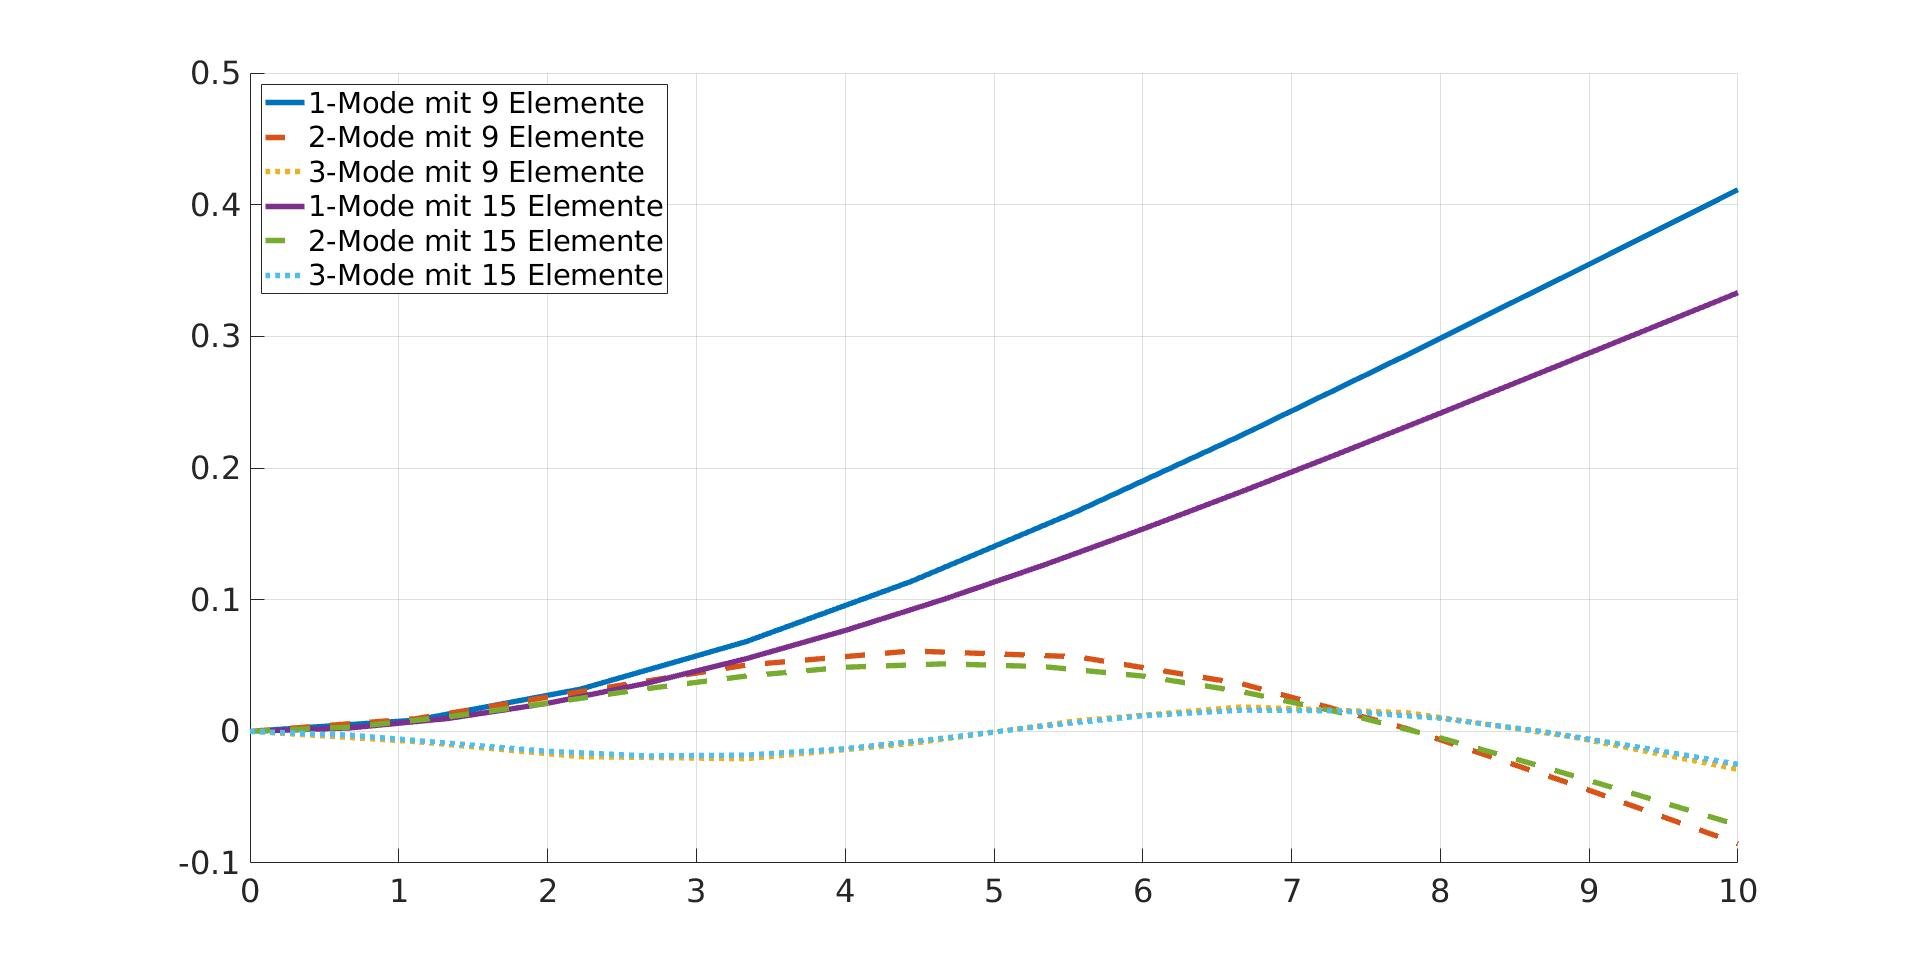
\includegraphics[width=1.1\linewidth, height=0.45\textheight]{Balken_9_15}
		\caption{Eigenschwingformen des Balkens mit unterschiedlicher Elementanzahl.}
		\label{fig:balken-9-15}
	\end{figure}

	
	\subsection{Biegeschwingungen einer Platte} \label{analysieren-platten}
	Es wird eine einseitig eingespannte Platte betrachtet. Die Länge der Platte ist $ L = 2 \, \text{m} $, die Breite $ B = 2 \, \text{m} $, die Dicke $ H= 0,01 \, \text{m} $, die Dichte $ \rho= 7850 \, \text{kg}/\text{m}^{3} $, der E-Modul $ E= 2,1\times10^{11} \, \text{N}/\text{m}^{2} $ und die Poissonzahl $ \nu = 0,3 $ . \\
Es werden die FE-Ergebnisse (\Matlab) mit denen aus \Ansys verglichen. In der folgenden Tabelle sind die verschiedenen Ergebnissen aufgelistet. Bei der Simulation mit \Matlab wird die Platte durch konforme Elemente diskretisiert mit je 9 oder 15 Elementen pro Seite. Bei der Simulation mit \Ansys wird jede Seite der Platte in 1000 Teile zerlegt.
	\begin{table}[H]\label{tab:platten-RB}
		\renewcommand\arraystretch{1.2}
		\centering
		\resizebox{\textwidth}{11mm}{		
		\begin{tabular}{|c|c|c|c|c|c|c|c|c|c|}
			\hline
			\diagbox[]{Eigenfrequenz [Hz]}{Mode}                              & 1        & 2        & 3         & 4         & 5         & 6         & 7         & 8         & 9         \\
			\hline
			 9 Elemente je Seite & 2,162105 & 5,299083 & 13,259113 & 16,940469 & 19,284920 & 33,759497 & 38,167191 & 39,961917 & 44,225406 \\
			\hline	
			15 Elemente je Seite & 2,161776 & 5,298090 & 13,256507 & 16,938819 & 19,280190 & 33,748742 & 38,150961 & 39,947782 & 44,201679\\
			\hline	 
			Ergebnis \Ansys & 2,161505 & 5,293666 & 13,254572 & 16,932654 & 19,265101 & 33,713487 & 38,157460 & 39,942079 & 44,185442 \\
			\hline
		\end{tabular}}
		\caption{Eigenfrequenzen der Biegeschwingungen einer einseitig eingespannten Platte.}
	\end{table}

	Es ist ersichtlich, dass die Genauigkeit des Eigenfrequenzen, im Vergleich zu \Ansys, von der Anzahl der Elemente abhängig ist. D.h. je mehr Elemente verwendet werden, desto besser ist das Ergebnis. Obwohl mehr Elemente die Genauigkeit der Ergebnisse steigern, ist die Simulation mit mehr Rechenzeit verbunden. Deshalb muss die Anzahl der Elemente richtig bestimmt werden, um eine schnellen Rechnung mit ausreichender Genauigkeit zu erreichen.

	Die Bilder \ref{fig:platten-RB-9} und \ref{fig:platten-RB-15} zeigen die verschiedenen Eigenschwingformen der einseitig eingespannten Platte, die durch die Simulation mit \Matlab berechnet und dargestellt wurden.
	\begin{figure}[H]
		\centering
		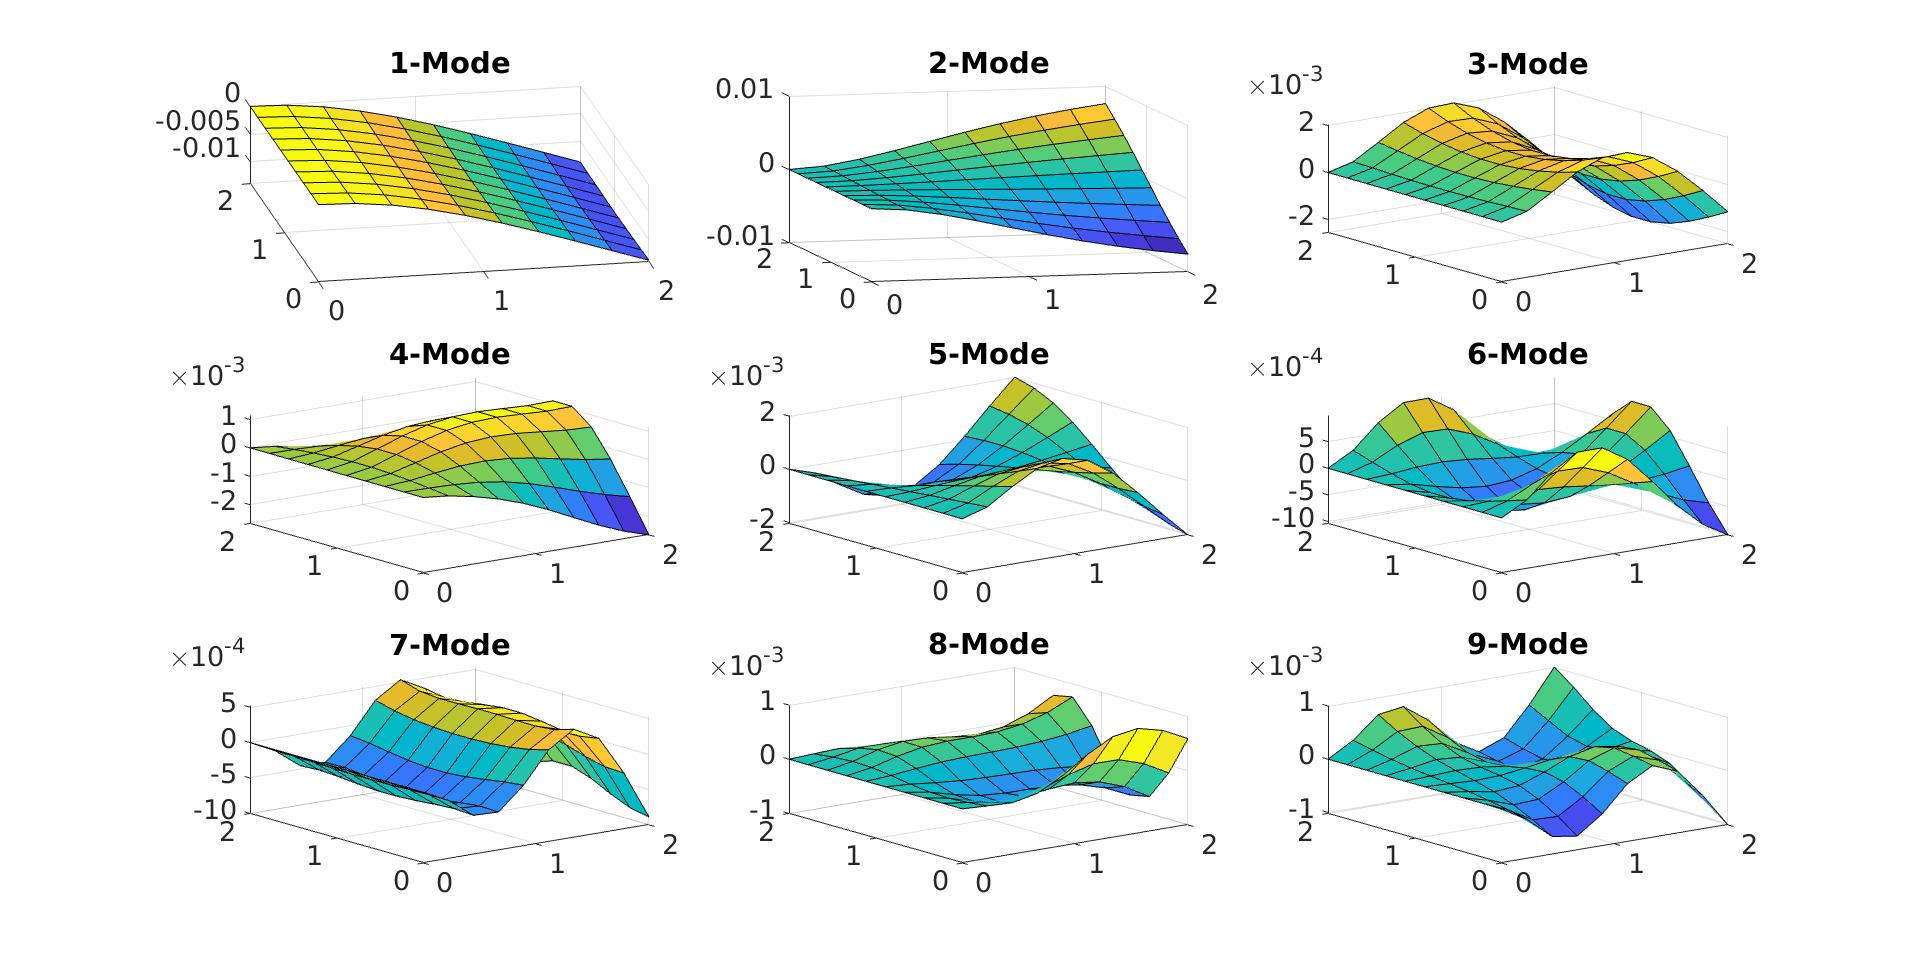
\includegraphics[width=1.0\linewidth]{Platten_RB_9}
		\caption{Eigenschwingformen einer einseitig eingespannten Platte mit 9 Elementen je Seite.}
		\label{fig:platten-RB-9}
	\end{figure}	
	\begin{figure}[H]
		\centering
		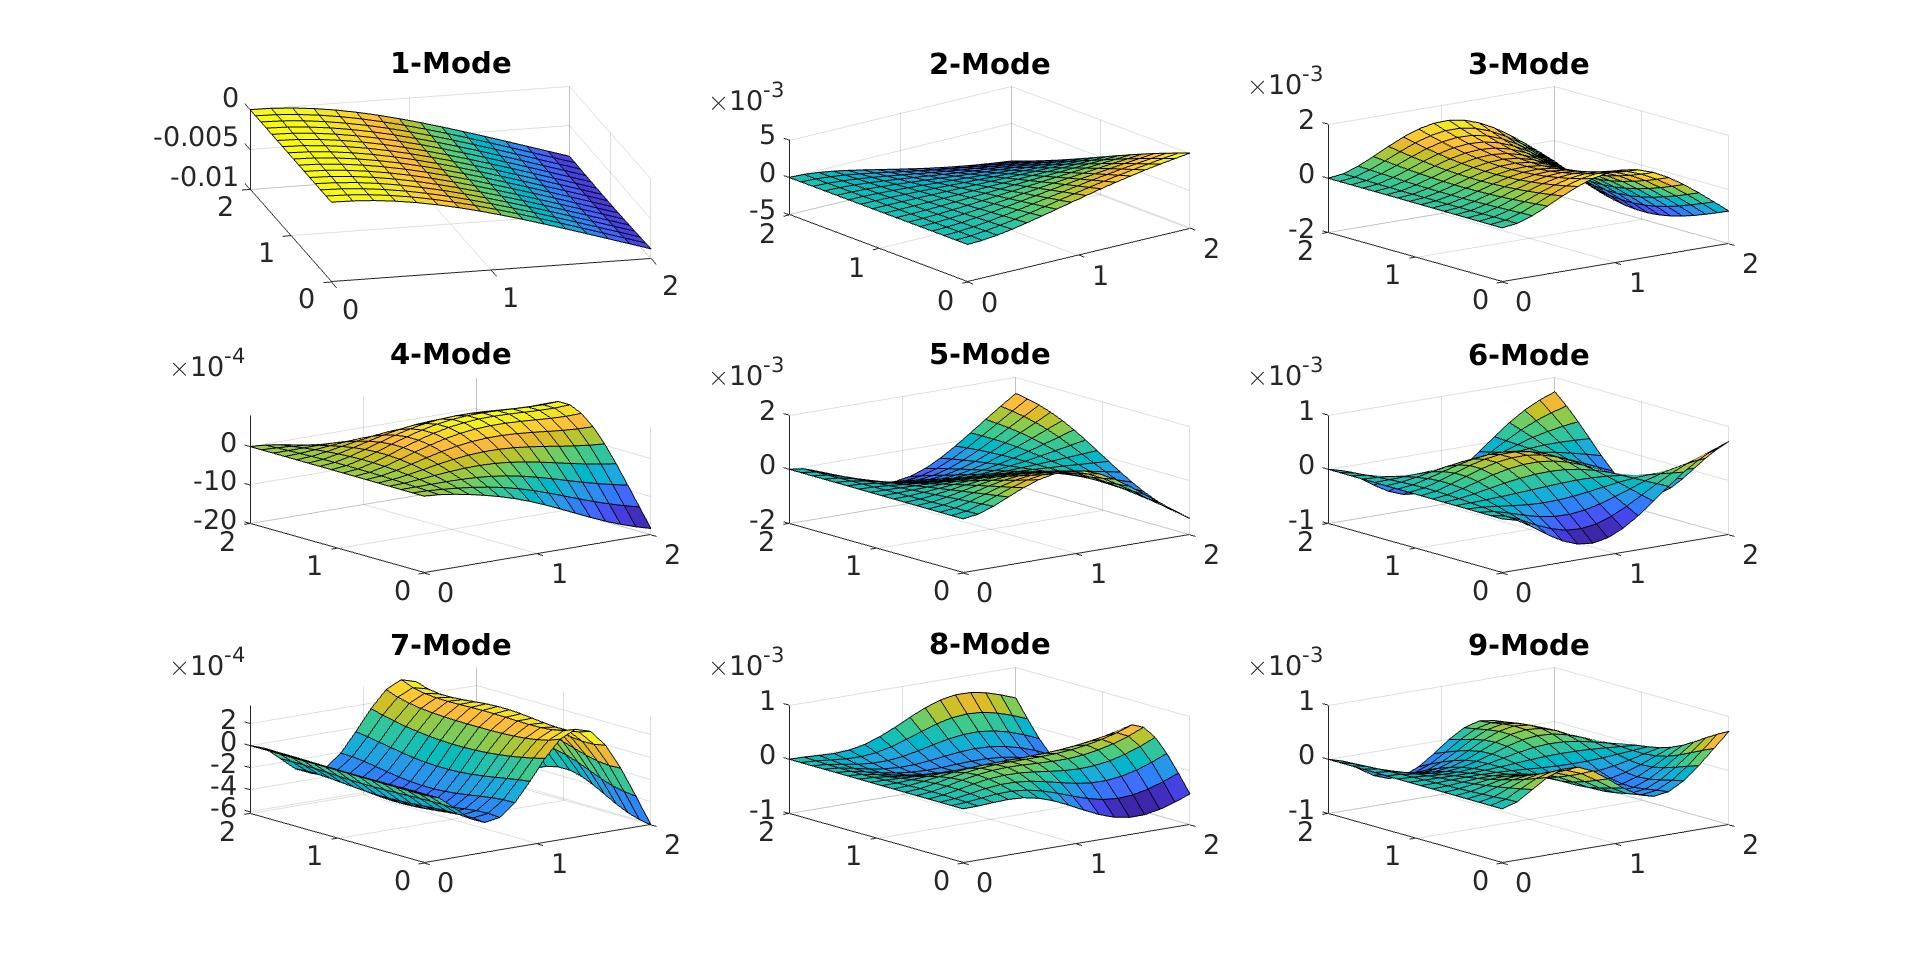
\includegraphics[width=1.0\linewidth]{Platten_RB_15}
		\caption{Eigenschwingformen einer einseitig eingespannten Platte mit 15 Elementen je Seite.}
		\label{fig:platten-RB-15}
	\end{figure}
	
	
	\clearpage
	\pagestyle{fancy}	
	\section{Zusammenfassung}
	Das Ziel der Modalanalyse besteht darin, eine Basis für die Identifizierung der modalen Parameter des Systems bereitzustellen. Die Analyse der Schwingungseigenschaften des strukturellen Systems dient zur Diagnose und Vorhersage von Vibrationsfehlern sowie der Optimierung der dynamischen Strukturmerkmale. Daher untersucht die Modalanalyse von Anfang an die Eigenschaften der Struktur. Das Verständnis der Eigenfrequenzen und der Eigenschwingformen hilft beim Entwurf eines Systems, das den Anforderungen von Lärm- und Vibrationsanwendungen entspricht.\\
	
	In dieser Arbeit wurde die numerische Modalanalyse mit der Finite-Elemente-Methode betrachtet. Die FE Simulationen wurde mit \Matlab durchgeführt und mit der kommerziellen Software \Ansys sowie analytischen Lösungen nach \cite{stephan1995schwingungen} verglichen. \\
	
	Durch die theoretischen Grundlagen wurden die numerischen Verfahren deutlich erklärt und das Fundament für die Simulationen gelegt. In den Simulationen wurden drei verschiedene Körper (Stab, Balken, Platte) betrachtet, die häufig im konstruktiven Ingenieurbau angewendet werden. Anhand der Ergebnisse lässt sich der Zusammenhang angeben, dass die Genauigkeit der Näherungslösung durch die Verwendung von immer mehr Parametern (z. B. mehr und mehr kleinere Elemente) oder Ansatzfunktionen mit immer höherem Wert verbessert werden kann.\\
	
	Darüber hinaus bedeuten immer mehr Parameter oder Ansatzfunktionen mit immer höherem Wert, dass die Simulationen mit mehr Rechenzeit verbunden sind. Deshalb muss die Anzahl der Elemente oder die Ansatzfunktionen problemorientiert berücksichtigt werden, um schnelle Rechnungen mit ausreichender Genauigkeit zu gewährleisten.\\
	
	Die Fehler der FE-Lösungen können auf unterschiedliche Gründe zurückgeführt werden. Vor allem sind die Anzahl der Elemente und die Ansatzfunktionen dafür verantwortlich. Außerdem gibt es numerische Fehler wie beispielsweise durch die Integralrechnung. Verschiedene Quadratur-Verfahren haben unterschiedliche numerische Genauigkeiten. In dieser Arbeit wurde nur die \textsc{Gauß}-Quadratur benutzt, da es sich um ein einfaches und schnelles Verfahren handelt. \\
	
	
	Durch die Erklärung der theoretischen Grundlagen und die Simulation von verschiedenen Körpern wurde die Modalanalyse für den eindimensionalen und zweidimensionalen Fall betrachtet. Da viele Probleme ein dreidimensionale Modell erfordern, kann als nächster Schritt dieser Fall betrachtet werden.
	\clearpage
	
%% empty page %%%%%%%%%%%%%%%%%%%%%%%%%%%%%%%%%%%%%%%%%%
	\newpage
	\pagestyle{empty}
	\ \\
	\newpage
%%%%%%%%%%%%%%%%%%%%%%%%%%%%%%%%%%%%%%%%%%%%%%%%%%%%%%%%%
	
	
	%\nocite{*}
	\pagestyle{fancy}
	\addcontentsline{toc}{section}{Quellenverzeichnis}
	\renewcommand{\refname}{Quellenverzeichnis}
	\bibliography{Projektarbeit}
	
	\clearpage
	
%% empty page %%%%%%%%%%%%%%%%%%%%%%%%%%%%%%%%%%%%%%%%%%
	\newpage
	\pagestyle{empty}
	\ \\
	\newpage
%%%%%%%%%%%%%%%%%%%%%%%%%%%%%%%%%%%%%%%%%%%%%%%%%%%%%%%%%
	
		\pagestyle{fancy}
	\fancyhead[RO,LE]{Anhang A: Programm Stabelemente}
	\setcounter{page}{1} 
	\fancyhead[LO,RE]{A-\thepage}
	%\specialsectioning
	\addcontentsline{toc}{paragraph}{Anhang A: Programm Stabelemente}
	\section*{Anhang A: Programm Stabelemente}
	\subsection*{Hauptprogramm linearer Ansatz}
	\begin{lstlisting}
	clear
	clc
	close
	%###########################################
	% main Program
	%###########################################
	% parameter
	E=2.1e11;           % N/m^2
	A=0.0001;           % m^2
	l=10;               % m
	rho=7850;           % Dichte in [kg/m^3]
	mu=rho*A;           % Massenbelegung in [kg/m]
	Nel=15;             % number of elements
	Nno=Nel+1;          % number of nodes
	le=l/Nel;           % length of an element
	
	% define empty matrice
	Kt=zeros(Nno);   % empty global stiffnes-matrix 
	M=zeros(Nno);    % empty global mass-matrix 
	
	% call element routinesmbclient
	[Kte,Me] = Elementroutine_linear(A,E,rho,le);
	
	% loop over every element
	for j=1:Nel  
	  M(j : j+1, j : j+1) = M(j : j+1, j : j+1) + Me;
	  Kt(j : j+1, j : j+1) = Kt(j : j+1, j : j+1)+ Kte;	
	end
	
	% implementation of essetial boundary conditions
	Kt(1,:) = [  ];
	Kt(:,1) = [  ];
	M(1,:)  = [  ];
	M(:,1)  = [  ];
	
	% define system-matrix
	null=zeros(size(M));
	Eins = eye(size(M));
	SysMat=[null,Eins; -inv(M)*Kt,null];
	
	% compute Eigenvalues
	[V,D]=eig(SysMat);
	temp_d = diag(D);
	[nd, sortindex] = sort(temp_d);
	temp_v = V(:,sortindex);
	temp_f = imag(nd)/(2*pi);
	
	% analysis method
	lamda = zeros(Nel, 1);
	omega = zeros(Nel, 1);
	f = zeros (Nel, 1);
	for k = 1: Nel
	 lamda (k) = (2 * k - 1 ) * pi /( 2 * l) ;
	 omega (k) = lamda(k)*sqrt(E/rho);
	 f(k) = omega(k)/(2*pi);
	end
	\end{lstlisting}

	\subsubsection*{Elementrechnung linearer Ansatz}
	\begin{lstlisting}
	%###########################################
	% Elementroutine
	%###########################################
	function [Kte,Me] = Elementroutine_linear(A,E,rho,le)
	% Elementroutine: compute Kte, Me
	% define empty Kte
	Kte=[0,0;0,0]; 
	% define empty Me 
	Me=[0,0;0,0];
	
	% define sampling points for Gauss-quadrature
	xiVec=[-sqrt(1/3),sqrt(1/3)];
	% weights for sampling points of Gauss-quadrature
	wVec =[1,1];  
	
	for i=1:length(xiVec)
	 xi=xiVec(i);
	  w=wVec(i);
	
	 % define N, B vector 
	 N=[0.5-xi/2  0.5+xi/2 ];
	 Nx=[-0.5  0.5]*(2/le);
	
	 % compute Kte and Me for sampling point of Gauss-integration
	 Me=Me + rho * A * ( N' * N ) * w;
	 Kte=Kte + E * A * ( Nx' * Nx ) * w;
	end
	
	end
	\end{lstlisting}
	
	\subsection*{Hauptprogramm quadratischer Ansatz}
	\begin{lstlisting}
	clear
	close
	clc
	%###########################################
	% main Program
	%###########################################
	% parameter
	E=2.1e11;           % N/m^2
	A=0.0001;           % m^2
	l=10;               % m
	rho=7850;           % Dichte in [kg/m^3]
	mu=rho*A;           % Massenbelegung in [kg/m]
	Nel=15;             % number of elements
	Nno=Nel*2+1;        % number of nodes
	le=l/Nel;           % length of an element
	
	% define empty matrice
	Kt=zeros(Nno);   % empty global stiffnes-matrix 
	M=zeros(Nno);    % empty global mass-matrix 
	
	% call element routinesmbclient
	[Kte,Me] = Elementroutine_quadra(A,E,mu,le);
	% loop over every element
	for j=1:2 : Nno-1                                    
	 M(j : j+2, j : j+2) = M(j : j+2, j : j+2) + Me;
	 Kt(j : j+2, j : j+2) = Kt(j : j+2, j : j+2)+ Kte;   
	end
	
	% implementation of essetial boundary conditions
	Kt(1,:) = [  ];
	Kt(:,1) = [  ];
	M(1,:)  = [  ];
	M(:,1)  = [  ];
	
	% define system-matrix
	null=zeros(size(M));
	Eins = eye(size(M));
	SysMat=[null,Eins;-inv(M)*Kt,null];
	
	% compute Eigenvalues
	[V,D]=eig(SysMat);
	temp_d = diag(D);
	[nd, sortindex] = sort(temp_d);
	temp_v = V(:,sortindex);
	temp_f = imag(nd)/(2*pi);
	
	% analysis method
	lamda = zeros(18, 1);
	omega = zeros(18, 1);
	f = zeros (18, 1);
	for k = 1: 18
	 lamda (k) = (2 * k - 1 ) * pi /( 2 * l) ;
	 omega (k) = lamda(k)*sqrt(E/rho);
	 f(k) = omega(k)/(2*pi);
	end
	\end{lstlisting}
	
	\subsubsection*{Elementrechnung quadratischer Ansatz}
	\begin{lstlisting}
	%###########################################
	% Elementroutine
	%###########################################
	function [Kte,Me] = Elementroutine_quadra(A,E,mu,le)
	% Elementroutine: compute Kte, Me
	% define empty Kte
	Kte=zeros(3); 
	% define empty Me 
	Me=zeros(3);
	
	% define sampling points for Gauss-quadrature
	xiVec=[-sqrt(1/3),sqrt(1/3)]; 
	% weights for sampling points of Gauss-quadrature 
	wVec =[1,1];   
	
	for i=1:length(xiVec)
	 xi=xiVec(i);
	 w=wVec(i);
	
	 % define N, B vector 
	 N=[xi^2/2-xi/2  1-xi^2  xi/2+xi^2/2];
	 Nx=[xi-0.5  -2*xi  0.5+xi]*(2/le);
	
	 % compute Kte and Me for sampling point of Gauss-integration
	 Me=Me + mu * (N' * N) * w;
	 Kte=Kte + E * A * (Nx' * Nx) * w;
	end
	
	end
	\end{lstlisting}
	
	\clearpage
	
	\setcounter{page}{1} 
	\fancyhead[LO,RE]{B-\thepage}
	\fancyhead[RO,LE]{Anhang B: Programm Balkenelemente}
	\addcontentsline{toc}{subparagraph}{Anhang B: Programm Balkenelemente}
	
	\section*{Anhang B: Programm Balkenelemente}
	\subsection*{Hauptprogramm kubischer Ansatz}
	\begin{lstlisting}
	clear
	clc
	close
	%###########################################
	% main Program
	%###########################################
	% parameter
	E=2.1e11;        % N/m^2
	A=0.0001;        % m^2
	l=10;            % m
	rho=7850;        % Dichte in [kg/m^3]
	mu=rho*A;        % Massenbelegung in [kg/m]
	Nel=15;         % number of elements
	Nno=Nel+1;       % number of nodes
	le=l/Nel;        % length of an element
	B=0.005;         % Breit von Balken
	H=0.02;          % Hoehe von Balken
	I=(B*(H^3))/12;  % Flaechentraegheitsmoment
	
	% define empty matrice
	Kt=zeros(Nno*2);  % empty global stiffnes-matrix 
	M=zeros(Nno*2);   % empty global mass-matrix 
	
	% call element routinesmbclient
	[Kte,Me] = Elementroutine_Balken(A,E,rho,le,I);
	
	% loop over every element
	for j=1: 2 : length(M)-2                                   
	 M(j : j+3, j : j+3) = M(j : j+3, j : j+3) + Me;
	 Kt(j : j+3, j : j+3) = Kt(j : j+3, j : j+3)+ Kte;
	end
	
	% implementation of essetial boundary conditions
	Kt(1,:) = [  ];
	Kt(:,1) = [  ];
	M(1,:)  = [  ];
	M(:,1)  = [  ];
	
	Kt(1,:) = [  ];
	Kt(:,1) = [  ];
	M(1,:)  = [  ];
	M(:,1)  = [  ];
	
	% define system-matrix
	null=zeros(size(M));
	Eins = eye(size(M));
	SysMat=[null,Eins; -inv(M)*Kt,null];
	
	% compute Eigenvalues
	[V,D]=eig(SysMat);
	
	temp_d = diag(D);
	[nd, sortindex] = sort(temp_d);
	temp_v = V(:,sortindex);
	temp_f = imag(nd)/(2*pi);
	
	for i=1:Nel*2
	 temp_f(i,:)=[];
	end
	% vector with node coordinates
	lVec = zeros (Nno, 1); 	
	for k = 1: Nno
	 lVec(k)=l/Nel*(k-1);
	end
	% delete lover part von eigenvectors
	EigMat=temp_v(1:length(M),:) ; 
	EigMat=imag(EigMat);
	% delete unnecessary rows 
	for k = 1: length(M)/2      
	 EigMat(1+k,:)=[];       
	end
	% delete unnecessary colums
	for k = 1: length(M)
	EigMat(:,k)=[];        
	end
	% fill up EigMat for first with zero displacement
	EigMat=[zeros(1,length(M));EigMat]; 
	
	figure
	hold on
	grid on
	plot(lVec,-EigMat(:,1),'LineWidth',4);
	plot(lVec,EigMat(:,2),'--','LineWidth',4);
	plot(lVec,EigMat(:,3),':','LineWidth',4);
	set(gca,'FontSize',24);
	legend('1-Mode', '2-Mode', '3-Mode','Location','northwest');
	
	% analysis method
	lamda = zeros(Nel, 1);
	omega = zeros(Nel, 1);
	f = zeros (Nel, 1);
	for k = 1: Nel
	 switch k
	  case 1 
	   lamda(k) = 1.87510 ;
	  case 2
	   lamda(k) = 4.69409 ;
	  case 3
	   lamda(k) = 7.85476 ;
	  case 4
	   lamda(k) = 10.99554;
	 end
	 if k >= 5
	 lamda(k) = ((2*k-1)*pi)/2 ;
	 end	
	 omega (k) = ((lamda(k))^2)*sqrt((E*I)/(rho*A*(l^4)));
	 f(k)=omega(k)/(2*pi);
	end
	\end{lstlisting}
	
	\subsubsection*{Elementrechnung kubischer Ansatz}
	\begin{lstlisting}
	%###########################################
	% Elementroutine
	%###########################################
	function [Kte,Me] = Elementroutine_Balken(A,E,rho,le,I)
	% Elementroutine: compute Kte, Me
	% define empty Kte
	Kte=zeros(4);
	% define empty Me 
	Me=zeros(4);
	% define sampling points for Gauss-quadrature
	xiVec=[-sqrt(3/5),0,sqrt(3/5)]; 
	% weights for sampling points of Gauss-quadrature
	wVec=[5/9,8/9,5/9];            
	for i=1:length(xiVec)
	 xi=xiVec(i);
	 w =wVec(i);
	 % zwei Freiheitsgrade
	 N = [1/2-(3*xi)/4+(xi^3)/4   1/4-xi/4-(xi^2)/4+(xi^3)/4   1/2+(3*xi)/4-(xi^3)/4   -1/4-xi/4+(xi^2)/4+(xi^3)/4];
	 Nxx = [(3*xi)/2   -1/2+(3*xi)/2   -(3*xi)/2   1/2+(3*xi)/2]*((2/le)^2);
	 % compute Kte and Me for sampling point of Gauss-integration
	 Me=Me + rho * A * (N' * N) * w;
	 Kte=Kte + E * I * (Nxx' * Nxx) * w;
	end
	
	end
	\end{lstlisting}
	
	\clearpage
	
	% empty page %%%%%%%%%%%%%%%%%%%%%%%%%%%%%%%%%%%%%%%%%%
	\newpage
	\pagestyle{empty}
	\ \\
	\newpage
	%%%%%%%%%%%%%%%%%%%%%%%%%%%%%%%%%%%%%%%%%%%%%%%%%%%%%%%%
	
	\setcounter{page}{1} 
	\pagestyle{fancy}
	\fancyhead[LO,RE]{C-\thepage}
	\fancyhead[RO,LE]{Anhang C: Programm Plattenelemente}
	\addcontentsline{toc}{part}{Anhang C: Programm Plattenelemente}
	\section*{Anhang C: Programm Plattenelemente}
	\subsection*{Hauptprogramm konforme Plattenelemente}
	\begin{lstlisting}
	clear
	clc
	close
	%###########################################
	% main Program
	%###########################################
	% parameter
	E=2.1e11;       % N/m^2
	A=0.0001;       % m^2
	L=2;            % m  length of plate
	B=2;            % m  wide of plate
	rho=7850;       % Dichte in [kg/m^3]
	mu=rho*A;       % Massenbelegung in [kg/m]
	Nelx=15;        % number of elements per rand
	Nely=15;
	Nnox=Nelx+1;    % number of nodes per rand
	Nnoy=Nely+1;
	Nel_all=Nelx * Nely;  % total elements
	Nno_all=Nnox * Nnoy;  % total nodes
	lex=L/Nelx;           % length of an element
	ley=B/Nely;
	H=0.01;         % m Dicke von Platte
	v=0.30;         % Poissionzahl
	
	% define empty matrice
	Kt=zeros(Nno_all*4);     % empty global stiffnes-matrix 
	M=zeros(Nno_all*4);      % empty global mass-matrix 
	
	% call element routinesmbclient
	[Kte,Me] = Elementroutine_Platten(H,E,rho,lex,ley,v);
	% loop over every element
	r=0;
	a=zeros(4,1);
	b=a;
	c=[1 5 9 13];
	d=[4 8 12 16];
	for j=1 : Nely                                  
	 for k=1:Nelx
	  a(1)=((j-1)*Nnox+k-1)*4+1;
	  b(1)=a(1)+3;
	  a(2)=((j-1)*Nnox+k)*4+1;
	  b(2)=a(2)+3;
	  a(3)=((j*Nnox)+k-1)*4+1;
	  b(3)=a(3)+3;
	  a(4)=((j*Nnox)+k)*4+1;
	  b(4)=a(4)+3;
	  for m=1:4
	   for n=1:4
	    M(a(m):b(m), a(n):b(n)) = M(a(m):b(m), a(n):b(n)) + Me(c(m):d(m),c(n):d(n));
	    Kt(a(m):b(m), a(n):b(n)) = Kt(a(m):b(m), a(n):b(n)) + Kte(c(m):d(m),c(n):d(n));
	   end
	  end
	 end
	end
	
	% implementation of essetial boundary conditions
	M(1:Nnox*4,:) = [];
	M(:,1:Nnox*4) = [];
	
	Kt(1:Nnox*4,:) = [];
	Kt(:,1:Nnox*4) = [];
	
	% define system-matrix
	null=zeros(size(M));
	Eins = eye(size(M));
	SysMat=[null,Eins; -inv(M)*Kt,null];
	
	% compute Eigenvalues
	[V,D]=eig(SysMat);
	
	temp_d = diag(D);
	[nd, sortindex] = sort(temp_d);
	temp_v = V(:,sortindex);
	temp_f = imag(nd)/(2*pi);
	
	%% Mode Plot
	% vector with node coordinates
	xVec = zeros (Nnox, 1);     
	yVec = zeros (Nnoy, 1); 
	for k = 1: Nnox
	 xVec(k)=L/Nelx*(k-1);    
	end
	
	for g = 1: Nnoy
	 yVec(g)=B/Nely*(g-1);    
	end
	
	% delete lover part von eigenvectors 
	EigMat=temp_v(1:length(M),:) ;   
	EigMat=imag(EigMat);
	% delete unnecessary rows 
	for k = 1: length(M)/4      
	 EigMat(1+k:1+k+2,:)=[];       
	end
	% delete unnecessary colums
	for k = 1: length(M)
	 EigMat(:,k)=[];         
	end
	% fill up EigMat
	p = zeros(Nnox,Nnoy-1,9);
	for i = 1:9
	 for j = 1:Nnoy-1
	  for k = 1:Nnox
	   p(k,j,i) = EigMat(k+(j-1)*Nnox,i);
	  end
	 end
	end
	
	for i = 1 : 9
	 p1(:,:,i) = [zeros(Nnox,1),p(:,:,i)];
	end
	
	figure
	hold on
	for k = 1:9
	 subplot(3,3,k);
	 surf(yVec,xVec,p1(:,:,k));
	 set(gca,'FontSize',20);
	 title([num2str(k),'-Mode']);
	end
	\end{lstlisting}
	
	\subsubsection*{Elementrechnung konforme Plattenelemente}
	\begin{lstlisting}
	%###########################################
	% Elementroutine
	%###########################################
	function [Kte,Me] = Elementroutine_Platten(H,E,rho,lex,ley,v)
	% Elementroutine: compute Kte, Me
	% define empty Kte
	Kte=zeros(16);
	
	% define empty Me
	Me=zeros(16);
	
	% define sampling points for Gauss-quadrature
	xiVec=[-sqrt(3/7+2/7*sqrt(6/5)),-sqrt(3/7-2/7*sqrt(6/5)),sqrt(3/7-2/7*sqrt(6/5)),sqrt(3/7+2/7*sqrt(6/5))];
	etaVec=[-sqrt(3/7+2/7*sqrt(6/5)),-sqrt(3/7-2/7*sqrt(6/5)),sqrt(3/7-2/7*sqrt(6/5)),sqrt(3/7+2/7*sqrt(6/5))];
	% weights for sampling points of Gauss-quadrature
	wVec=[(18-sqrt(30))/36,(18+sqrt(30))/36,(18+sqrt(30))/36,(18-sqrt(30))/36];
	uVec=wVec;
	
	for i=1:length(xiVec)
	 x = xiVec(i);
	 w = wVec(i);
	 for j = 1:length(etaVec)
	  y = etaVec(j);
	  u = uVec(j);        
	  % define N, Nxx, Nyy, Nxy vector
	N=[ (1/16)*(-1 + x)^2*(2 + x)*(-1 + y)^2*(2 + y)  ...
	(1/16)*(-1 + x)^2*(1 + x)*(-1 + y)^2*(2 + y)  ...
	(1/16)*(-1 + x)^2*(2 + x)*(-1 + y)^2*(1 + y)  ...
	(1/16)*(-1 + x)^2*(1 + x)*(-1 + y)^2*(1 + y) ...
	(-(1/16))*(-2 + x)*(1 + x)^2*(-1 + y)^2*(2 + y) ...
	(1/16)*(-1 + x)*(1 + x)^2*(-1 + y)^2*(2 + y) ...
	(-(1/16))*(-2 + x)*(1 + x)^2*(-1 + y)^2*(1 + y) ...
	(1/16)*(-1 + x)*(1 + x)^2*(-1 + y)^2*(1 + y) ...
	(-(1/16))*(-1 + x)^2*(2 + x)*(-2 + y)*(1 + y)^2 ...
	(-(1/16))*(-1 + x)^2*(1 + x)*(-2 + y)*(1 + y)^2 ...
	(1/16)*(-1 + x)^2*(2 + x)*(-1 + y)*(1 + y)^2 ...
	(1/16)*(-1 + x)^2*(1 + x)*(-1 + y)*(1 + y)^2 ...
	(1/16)*(-2 + x)*(1 + x)^2*(-2 + y)*(1 + y)^2 ...
	(-(1/16))*(-1 + x)*(1 + x)^2*(-2 + y)*(1 + y)^2 ...
	(-(1/16))*(-2 + x)*(1 + x)^2*(-1 + y)*(1 + y)^2 ...
	(1/16)*(-1 + x)*(1 + x)^2*(-1 + y)*(1 + y)^2 ];
	
	Nxx=[ (3*x*(-1 + y)^2*(2 + y))/(2*lex^2) ...
	((-1 + 3*x)*(-1 + y)^2*(2 + y))/(2*lex^2) ...
	(3*x*(-1 + y)^2*(1 + y))/(2*lex^2) ...
	((-1 + 3*x)*(-1 + y)^2*(1 + y))/(2*lex^2) ...
	-((3*x*(-1 + y)^2*(2 + y))/(2*lex^2)) ...
	((1 + 3*x)*(-1 + y)^2*(2 + y))/(2*lex^2) ...
	-((3*x*(-1 + y)^2*(1 + y))/(2*lex^2)) ...
	((1 + 3*x)*(-1 + y)^2*(1 + y))/(2*lex^2) ...
	-((3*x*(-2 + y)*(1 + y)^2)/(2*lex^2)) ...
	-(((-1 + 3*x)*(-2 + y)*(1 + y)^2)/(2*lex^2)) ...
	(3*x*(-1 + y)*(1 + y)^2)/(2*lex^2) ...
	((-1 + 3*x)*(-1 + y)*(1 + y)^2)/(2*lex^2) ...
	(3*x*(-2 + y)*(1 + y)^2)/(2*lex^2) ...
	-(((1 + 3*x)*(-2 + y)*(1 + y)^2)/(2*lex^2)) ...
	-((3*x*(-1 + y)*(1 + y)^2)/(2*lex^2)) ...
	((1 + 3*x)*(-1 + y)*(1 + y)^2)/(2*lex^2) ];
	
	Nyy=[ (3*(-1 + x)^2*(2 + x)*y)/(2*ley^2) ...
	(3*(-1 + x)^2*(1 + x)*y)/(2*ley^2) ...
	((-1 + x)^2*(2 + x)*(-1 + 3*y))/(2*ley^2) ...
	((-1 + x)^2*(1 + x)*(-1 + 3*y))/(2*ley^2) ...
	-((3*(-2 + x)*(1 + x)^2*y)/(2*ley^2)) ...
	(3*(-1 + x)*(1 + x)^2*y)/(2*ley^2) ...
	-(((-2 + x)*(1 + x)^2*(-1 + 3*y))/(2*ley^2)) ...
	((-1 + x)*(1 + x)^2*(-1 + 3*y))/(2*ley^2) ...
	-((3*(-1 + x)^2*(2 + x)*y)/(2*ley^2)) ...
	-((3*(-1 + x)^2*(1 + x)*y)/(2*ley^2)) ...
	((-1 + x)^2*(2 + x)*(1 + 3*y))/(2*ley^2) ...
	((-1 + x)^2*(1 + x)*(1 + 3*y))/(2*ley^2) ...
	(3*(-2 + x)*(1 + x)^2*y)/(2*ley^2) ...
	-((3*(-1 + x)*(1 + x)^2*y)/(2*ley^2)) ...
	-(((-2 + x)*(1 + x)^2*(1 + 3*y))/(2*ley^2)) ...
	((-1 + x)*(1 + x)^2*(1 + 3*y))/(2*ley^2) ];
	
	Nxy=[ (9*(-1 + x^2)*(-1 + y^2))/(4*lex*ley) ...
	(3*(-1 + x)*(1 + 3*x)*(-1 + y^2))/(4*lex*ley) ...
	(3*(-1 + x^2)*(-1 + y)*(1 + 3*y))/(4*lex*ley) ...
	((-1 + x)*(1 + 3*x)*(-1 + y)*(1 + 3*y))/(4*lex*ley) ...
	-((9*(-1 + x^2)*(-1 + y^2))/(4*lex*ley)) ...
	(3*(1 + x)*(-1 + 3*x)*(-1 + y^2))/(4*lex*ley) ...
	-((3*(-1 + x^2)*(-1 + y)*(1 + 3*y))/(4*lex*ley)) ...
	((1 + x)*(-1 + 3*x)*(-1 + y)*(1 + 3*y))/(4*lex*ley) ...
	-((9*(-1 + x^2)*(-1 + y^2))/(4*lex*ley)) ...
	-((3*(-1 + x)*(1 + 3*x)*(-1 + y^2))/(4*lex*ley)) ...
	(3*(-1 + x^2)*(1 + y)*(-1 + 3*y))/(4*lex*ley) ...
	((-1 + x)*(1 + 3*x)*(1 + y)*(-1 + 3*y))/(4*lex*ley) ...
	(9*(-1 + x^2)*(-1 + y^2))/(4*lex*ley) ...
	-((3*(1 + x)*(-1 + 3*x)*(-1 + y^2))/(4*lex*ley)) ...
	-((3*(-1 + x^2)*(1 + y)*(-1 + 3*y))/(4*lex*ley)) ...
	((1 + x)*(-1 + 3*x)*(1 + y)*(-1 + 3*y))/(4*lex*ley) ];
	
	 % compute Kte and Me for sampling point of Gauss-integration
	 Me=Me + rho * H * (N' * N) * w * u;
	 Kte=Kte + ((E*H^3)/(12*(1-v^2))) * ((Nxx' * Nxx)+v*((Nxx'*Nyy)+(Nyy'*Nxx))+(Nyy'*Nyy)+2*(1-v)*(Nxy'*Nxy)) * w * u;
	 end
	 end
	
	end
	\end{lstlisting}
	
	
\end{document}